\documentclass[]{article}

\usepackage{graphicx, float}
\usepackage{caption}
\usepackage{subcaption}
\usepackage{gensymb}

\usepackage{amsmath,amsfonts,amsthm,amssymb}
\usepackage[cal=cm]{mathalfa}

\newtheorem{mydef}{Definition}
\newtheorem{myprop}{Property}
\newtheorem{mythm}{Theorem}
\newtheorem{mylem}{Lemma}

\graphicspath{{./Figures/}}

%opening
\title{Penrose Aperiodic Tiling of the Plane and Collins' Paths}
\author{Jesse Bettencourt}

\begin{document}

\maketitle

\section{Introduction to Tessellations}
\subsection{Definitions}
We will begin our discussion of Penrose tilings with some definitions given by Senechal \cite{Senechal1996}. First, a formal definition of a tiling of Euclidean n-space, $\mathbb{E}^n$:



\begin{mydef}
A \textbf{tiling} $\mathcal{T}$ of the space $\mathbb{E}^n$ is a countable family of closed sets, $T$, called tiles:
\begin{equation*}
\mathcal{T}=\{T_1,T_2,\mathellipsis\}
\end{equation*}
such that
\begin{enumerate}
\item $\mathcal{T}$ has no overlaps: $\mathring{T_i} \cap \mathring{T_j}=\emptyset$ if $i\neq j$
\item $\mathcal{T}$ has no gaps: $\bigcup_{i=1}^\infty T_i = \mathbb{E}^n$
\end{enumerate}
\end{mydef}


Here $\mathring{T}$ denotes the interior of tile $T$. Further, we assume that a tile is the closure of its interior, and that tiles have positive volume. These assumptions allow, for example, a line segment to be a tile in $\mathbb{E}^1$ but not in $\mathbb{E}^2$. Notice that this definition of tiling neither restricts the shape of the individual tiles nor the number of unique tiling shapes.  

However, we will impose some restrictions on the tiles here. Since we are considering tilings of the plane, our tiling must satisfy the above definition for $n=2$, that is, for the Euclidean plane $\mathbb{E}^2$. Further, while the general definition does not impose any criteria on tile shape, for our purposes we will only consider n-dimensional polytopes. In the case of the plane, we consider only 2-polytopes, or polygons. To denote the facets of our tiles we will use \textbf{edges} to denote the 1-dimensional faces, and \textbf{vertices} to denote the 0-dimensional faces. 

\begin{mydef}
Let $\{T_1,T_2,\mathellipsis\}$ be the set of tiles of tiling $\mathcal{T}$, partitioned into a set of equivalence classes by criterion $\mathcal{M}$. The set, $\mathcal{P}$, of representatives of these equivalence classes is called the \textbf{protoset} for $\mathcal{T}$ with respect to $\mathcal{M}$.
\end{mydef}

For example, consider an infinite black-and-white checkerboard (Fig.\ref{fig:checkerboard}). Each tile in the checkerboard is either a black or white square, and the tiling is given by the matching rule that black squares may only share edges with white squares, and vice-versa. In this example, the equivalence class criterion, $\mathcal{M}$, is the colour of the square together with this matching rule. The protoset, $\mathcal{P}$, for the checkerboard is the set containing two elements: a black square and a white square.

\begin{figure}[H]

  \hspace*{\fill}
\begin{subfigure}[t]{0.4\textwidth}
	\includegraphics[width=\textwidth]{Checkerboard}
    \caption{Checkerboard}
    \label{fig:checkerboard}
\end{subfigure}
  \hspace*{\fill}
\begin{subfigure}[t]{0.4\textwidth}
	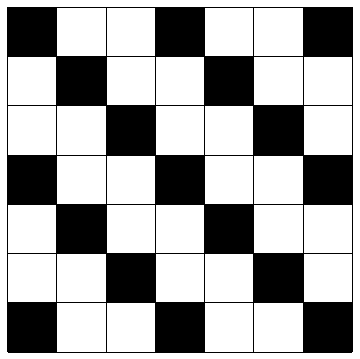
\includegraphics[width=\textwidth]{CheckerboardOther}
    \caption{Different Criterion.}
    \label{fig:critchecker}
\end{subfigure}
  \hspace*{\fill}\\
  \hspace*{\fill}
  \begin{subfigure}[t]{0.4\textwidth}
  	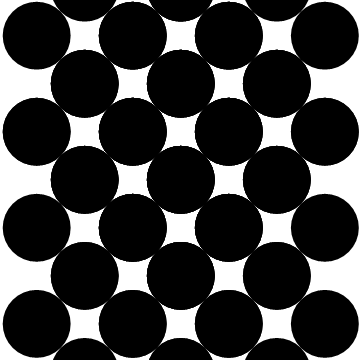
\includegraphics[width=\textwidth]{CheckerboardCircles}
      \caption{Deformed Checkerboard}
      \label{fig:deformedchecker}
  \end{subfigure}
      \hspace*{\fill} 
\begin{subfigure}[t]{0.4\textwidth}
	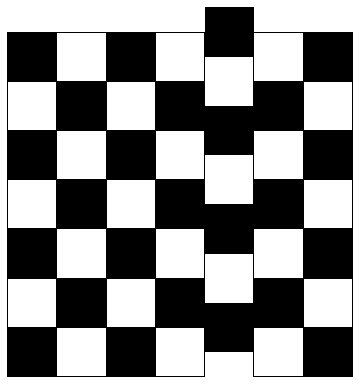
\includegraphics[width=\textwidth]{CheckerboardAperiodic}
    \caption{Sub-Periodic Checkerboard}
    \label{fig:aperiodicchecker}
\end{subfigure} 
\hspace*{\fill}
\label{fig:checker}
\caption{A protoset of black and white squares can admit multiple tilings. Some of them may be periodic, but this is not necessary.}
\end{figure}

\begin{mydef}
If $\mathcal{T}$ is a tiling with protoset $\mathcal{P}$, then we say that $\mathcal{P}$ admits $\mathcal{T}$.
\end{mydef}

In the checkerboard example we say that the protoset containing black and white squares, together with the matching criterion, admits a checkerboard tiling (Fig.\ref{fig:checkerboard}). It is important to note that a protoset can admit multiple tilings given different criterion. For example, the checkerboard protoset also admits the tiling in Fig.\ref{fig:critchecker} under a different matching rule. 

Further, it is also worth noting that abstract criterion, such as colour-matching or directed edges, can be accomplished instead through deformation of the edges of protoset tiles such that the criterion is forced. Consider again the criterion for producing the checkerboard tiling (Fig.\ref{fig:checkerboard}), that black squares may only share edges with white squares, and vice-versa. One way to realize this criterion is to deform all black squares into circles, and to deform white squares into curved diamonds. As seen in Fig.\ref{fig:deformedchecker}, these deformations force a tiling such that all white tiles occupy the interstices of the black circles. In other words, the protoset of deformed tiles, the black circle and white curved diamond, can only admit one unique tiling. We are able to force a checkerboard patter without any abstract criterion such as colour-matching adjacent tiles. While it is important to understand that abstract matching criterion can be realized by edge deformations, considering simpler protosets with more complicated criterion will usually allow greater insight into the structure and patterns within a tiling than would considering a simple criterion with complicated prototiles. 

\begin{mydef}
A tiling of  $\mathbb{E}^n$ is said to be \textbf{periodic} if it admits translational symmetry in $n$ linearly independent directions.
\end{mydef}

For example, the checkerboard tiling in Fig.\ref{fig:checkerboard} is periodic, as it has translational symmetry in two directions: vertical translation by two units, and horizontal translation by two units. Likewise, we can see that the criterion generating Fig.\ref{fig:critchecker} produces a tiling which is also periodic, with vertical and horizontal translational symmetry given by translation by three units. 

\begin{mydef}
A tiling of  $\mathbb{E}^n$ is said to be \textbf{sub-periodic} if it admits translational symmetry in $k$ linearly independent directions, where $1\leq k\leq n$. A tiling is said to be \textbf{non-periodic} if it admits no translational symmetry. 
\end{mydef}

For example, consider the checkerboard pattern with a single `column' translated vertically by a half-unit distance (Fig.\ref{fig:aperiodicchecker}). This tiling admits translational symmetry in the vertical direction with translation by two units. However, we can see that there is no horizontal symmetry because horizontal translation will not allow the shifted column to overlap anywhere. For this reason, there are also no diagonal translational symmetries admitted. This column shifted checkerboard is sub-periodic. 

We've seen that the protoset of black and white squares admits multiple types of tiling, both periodic and sub-periodic. Some protosets, such as the circle and curved diamond (Fig.\ref{fig:deformedchecker}), admits tilings which are only periodic. A question which motivated the discovery of the Penrose tiles was whether we can find protosets that admit \textit{only} non-periodic tilings.

\begin{mydef}
A protoset $\mathcal{P}$ is said to be \textbf{aperiodic} if it admits only non-periodic tilings. A tiling $\mathcal{T}$ from an aperiodic protoset is called an \textbf{aperiodic tiling}. 
\end{mydef}

Here, `only' means that no subset of the protoset, nor the entire protoset, can tile periodically. 


\subsection{Kepler's Monsters}


\subsection{Discovering Aperiodic Tessellations}
Studied in the mid-1900's was a class of tilings produced by arranging isosceles to radially spiral about a central point. A method discovered by Micheal Goldberg in 1955 produces these spiral tilings readily. Further, due to their spiraling arrangement, these tilings admit no translational symmetries, so non-periodic. However, these spiral tilings are produced by a protoset which also admits periodic tilings. In fact, all other non-periodic tilings known at the time, notably Golomb's `reptiles', were formed from protosets which also admit periodic tilings.

It was widely conjectured that no protosets existed which allow only non-periodic tiling. That is, that no aperiodic protosets were possible. This was proved untrue when, in 1961, Hao Wang began writing on protosets composed of unit squares with coloured edges, called Wang dominoes. The matching rules for these dominoes require adjacent dominoes to share the same colour on their abutting edge, with rotation and reflection not allowed. Wang was concerned with questions in logic, specifically investigating procedures for deciding whether any arbitrary set of dominoes would admit a plane tiling, called decision procedures. Wang posed a conjecture that any protoset which can admit a plane tiling will also admit a periodic tiling, and Wang showed that if this is true then there must also be a procedure for deciding whether such a set will tile. 

In 1964, Robert Berger showed in his doctoral thesis from Harvard University that Wang's conjecture is false, that there is no decision procedure for any arbitrary protoset. The implication of Berger's work is that there must be an aperiodic protoset of Wang dominoes. Further, Berger constructed this protoset, using 20,426 dominoes. In his later work, Berger produced a smaller protoset, using only 104 dominoes. Donald Knuth further reduced this number by finding an aperiodic Wang protoset of only 92 tiles.

As discussed previously, tiling matching rules can be realized by deformations on the edges of the prototiles. For instance, instead of the coloured edges of the Wang dominoes, consider deforming the edges of the squares into protrusions and cavities, producing prototiles like pieces of a jigsaw puzzle. These deformations can be chosen in such a way that they permit only the same arrangements as did the coloured edges of the dominoes, however, this representation also allows for rotation and reflection of the prototiles. 

By representing the protoset as described above, Raphael Robinson constructed in 1971 an aperiodic protoset requiring only six prototiles. The prototiles used by Robinson are considered to still be in the category of `square' tiles, and whether size of an aperiodic protoset of square tiles can be reduced to fewer than six tiles is still unknown. However, it is conjectured that six is the minimum number of square aperiodic protosets. This was supported in 1977 when Robert Ammann found a different aperiodic protoset of six square prototiles.

In 1973, Roger Penrose found an aperiodic protoset of six, non-square tiles. In 1974, Penrose reduced this number to four, and shortly after reduced them further to two. There are arbitrarily many representations of these two prototiles, but twp representations are considered simplest and most recognizable. 

The first of these representations, the Penrose Rhombs, is a set of two rhombi with equal lengths, but different internal angles. The thin rhombus, \textbf{t}, has corner angles of $\frac{\pi}{5}$ and $\frac{4 \pi}{5}$ (or $36 \degree$ and $144 \degree$). The thick rhombus, \textbf{T}, has corner angles  $\frac{2 \pi}{5}$ and $\frac{3 \pi}{5}$ (or $72 \degree$ and $108 \degree$). Both thin and thick rhombi can be produced by the composition of Robinson's Golden triangles, named after Robinson's 1975 notes. The rhombs can be produced by reflecting the isosceles Robinson triangles across their bases. The ratio of the leg and base lengths in the Robinson triangles is the Golden Ratio, \textbf{ $\phi= \frac{1+\sqrt{5}}{2}\approx 1.6180$}. This ratio will appear repeatedly throughout this discussion of Penrose tilings. 

The other common representation of Penrose's tiles is the Kite and Dart protoset, named by John Conway. These prototiles are also produced by the composition of Robinson triangles, rather by reflection across their legs. 

Neither the Rhombs nor the Kites and Darts tilings were publicized until after Penrose filed for patents on the shapes, due to their commercial potential as board game puzzles. It was Martin Gardner who finally published Penrose and Conway's work on describing these tilings, as well as their method of constructing the tiling by substitution, in his 1977 ``Mathematical Games'' column in \textit{Scientific American}. 

In 1981, Dutch mathematician Nicolaas de Bruijn provided other methods of constructing the Penrose tiling, by projecting of five-dimensional cubic structure and also by infinite paths on directed graphs, which will discussed later. De Bruijn also showed the relationship between the Penrose tiling and five families of parallel lines, called the Pentagrid. De Bruijn's work represents the characterization of Penrose tilings as algebraic objects, and offers deep insight into their nature. 

The practical importance of these theories on aperiodic tiling was realized in the 1980's with the discovery by materials scientist Dan Shechtman of certain aluminum-manganese alloys which produce crystallographic diffraction patterns with no translational symmetries. Shechtman was awarded the 2011 Nobel Prize in Chemistry for his discovery of these structures, known now as quasicrystals. In 2009, the first natural quasicrystal was discovered, the mineral icosahedrite, whose diffraction pattern displays fivefold symmetry previously thought impossible in crystalline structures. This past month, in March 2015, the second natural quasicrystal was discovered in a meteorite, with a diffraction pattern displaying decagonal symmetry \cite{Bindi2015}. Marjorie Senechal formalizes the relationship between aperiodic tiling and the geometry of quasicrystals in her 1995 monograph \textit{Quasicrystals and Geometry}. 


\section{The Penrose Tiling}
\subsection{Rhombus Representation of the Penrose Tiling}
As introduced, there are many protoset representations which admit the Penrose tilings. For the purposes of this discussion, we will focus mostly on the Penrose Rhombs (see Fig.\ref{fig:Rhombs}). 

Since this protoset is composed of two rhombi, it might be suspected that the prototiles can be arranged to produce a periodic tiling, since rhombi can generally produce periodic tilings. Consider, for example, the tiling produced by adjacent rows of thick and thin rhombi (see Fig.\ref{fig:RhombsPeriodic}). This tiling underscores the necessity of edge-matching rules for the aperiodic protoset. 

The edge-matching rules of the Penrose rhombs have been illustrated with blue and orange curves in Fig.\ref{fig:Rhombs}. If two tiles are adjacent in a tiling, then curves of the same colour must meet along the abutting edge. For example, the previously discussed periodic rhombus tiling is not permitted given this edge-matching criteria, because these curves do not meet along adjacent tiles (see Fig.\ref{fig:RhombsPeriodicRules}). Further, recall from previous description that matching criteria can be realized through prototile edge deformations (see Fig.\ref{fig:deformedchecker}). This allows us to consider the Rhombs protoset with matching rules as distinct from the Rhombs without matching rules, permitting us to describe the former as aperiodic. 


\begin{figure}[H]
\begin{subfigure}[t]{0.4\textwidth}
\centering
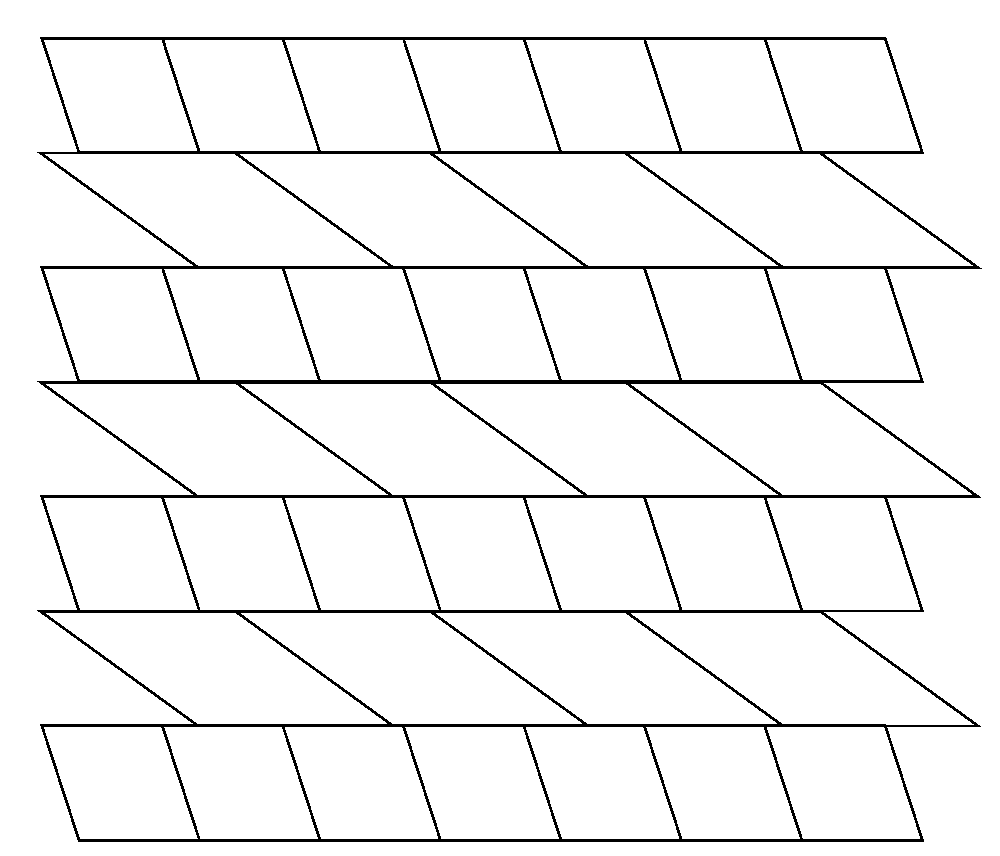
\includegraphics[width=\textwidth]{RhombPeriodic}
\caption{Periodic tiling of thin and thick rhombi, admitted in the absence of edge-matching rules.}
\label{fig:RhombsPeriodic}
\end{subfigure}\hfill
\begin{subfigure}[t]{0.4\textwidth}
\centering
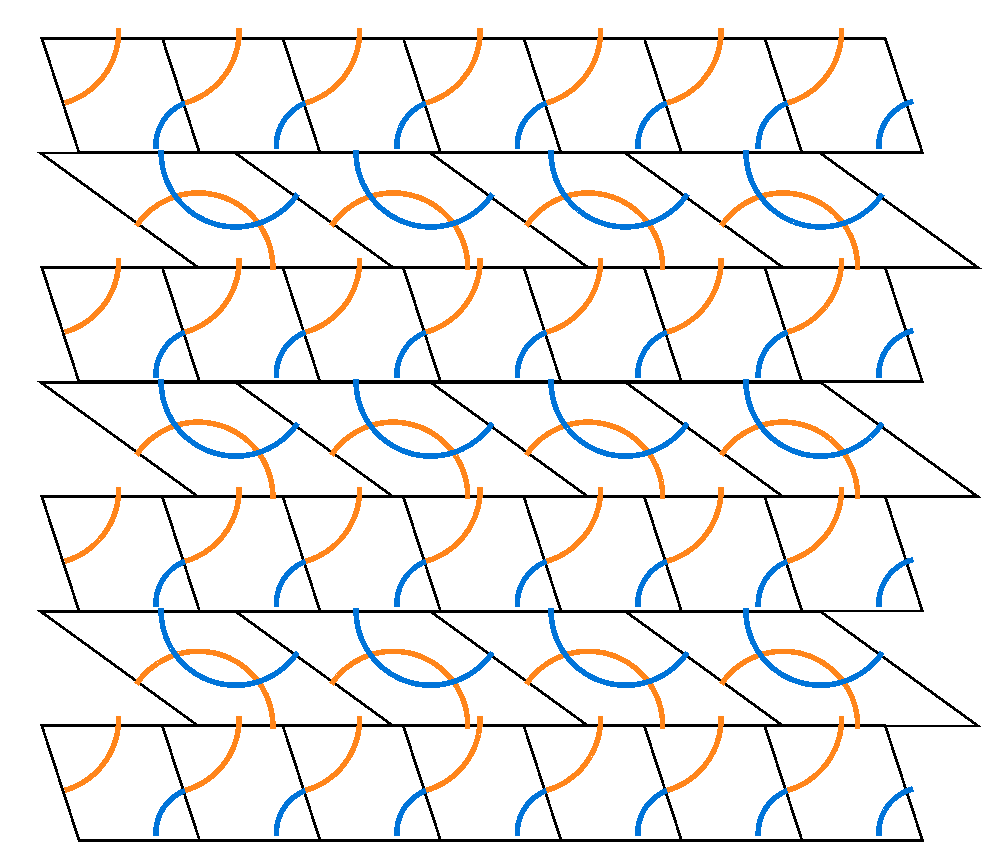
\includegraphics[width=\textwidth]{RhombPeriodicRules}
\caption{Matching rules require blue and orange curves to meet along adjacent edges. Clearly, this tiling does not satisfy these matching rules.}
\label{fig:RhombsPeriodicRules}
\end{subfigure}
\caption{Periodic tiling using Penrose rhombs is only possible in the absence of edge-matching rules.}

\end{figure}

\begin{figure}
        \centering
        \begin{subfigure}[b]{\textwidth}
        \begin{subfigure}[b]{0.5\textwidth}
                \centering
                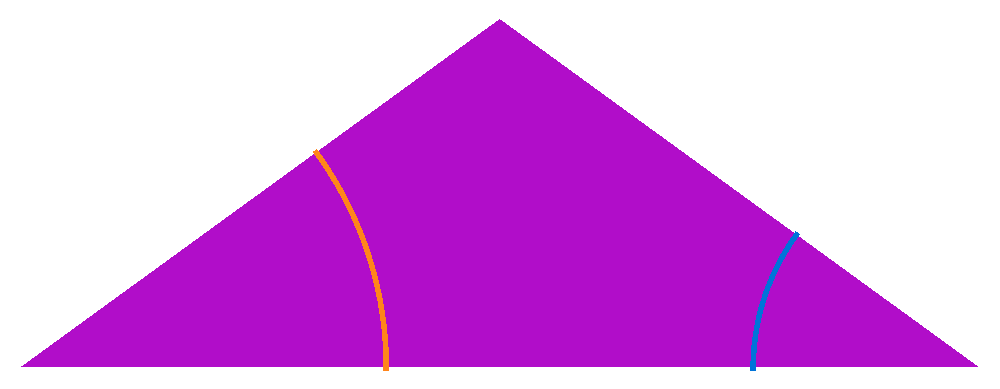
\includegraphics[scale=0.5]{RobinsonFat}
                \subcaption{Thick Robinson Triangle}
                \label{fig:RobThick}
        \end{subfigure}\hfill%
        ~ %add desired spacing between images, e. g. ~, \quad, \qquad, \hfill etc.
          %(or a blank line to force the subfigure onto a new line)
        \begin{subfigure}[b]{0.5\textwidth}
                \centering
                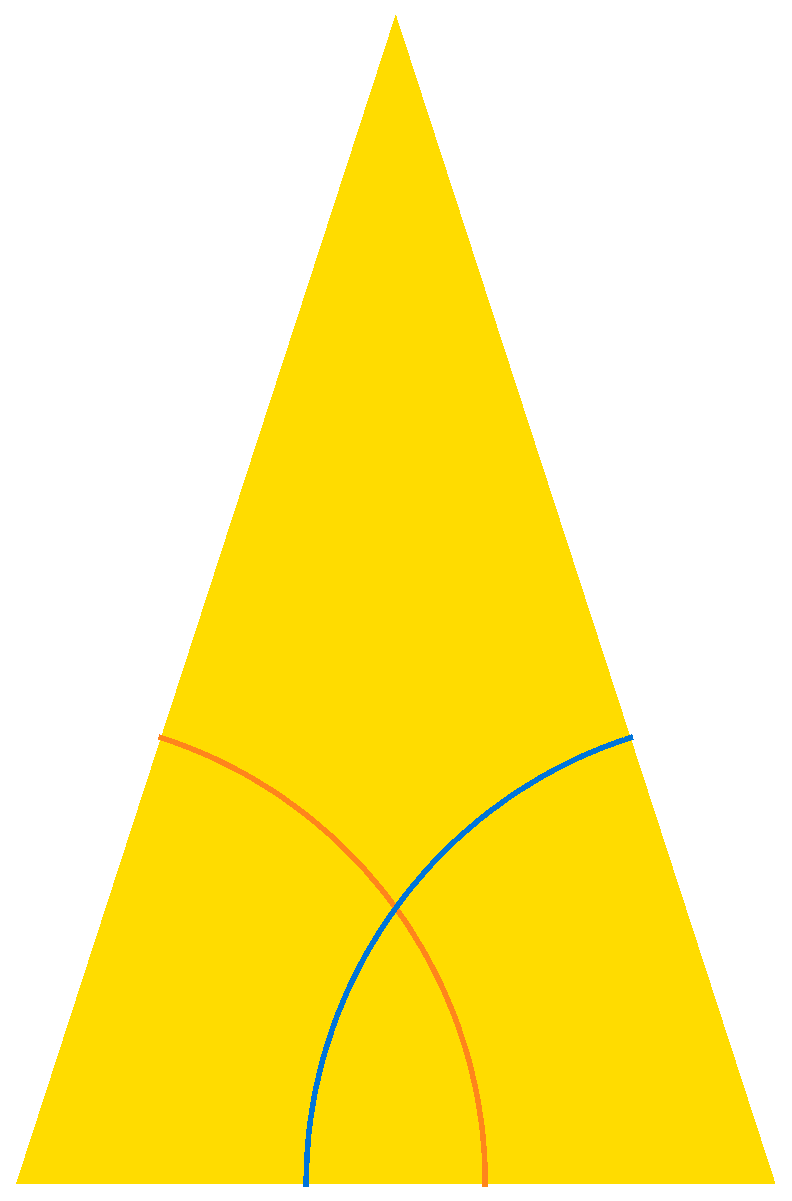
\includegraphics[scale=0.3]{RobinsonSkinny}
                \subcaption{Thin Robinson Triangle}
                \label{fig:RobThin}
        \end{subfigure}
        \caption*{Robinson Triangles with Golden leg-to-base ratio, $\phi$.}
        \label{fig:RobTris}
        \end{subfigure}
        ~ %add desired spacing between images, e. g. ~, \quad, \qquad, \hfill etc.
          %(or a blank line to force the subfigure onto a new line)
          
        \begin{subfigure}[b]{\textwidth}
        \begin{subfigure}[b]{0.5\textwidth}
        \centering
                \raisebox{40px}{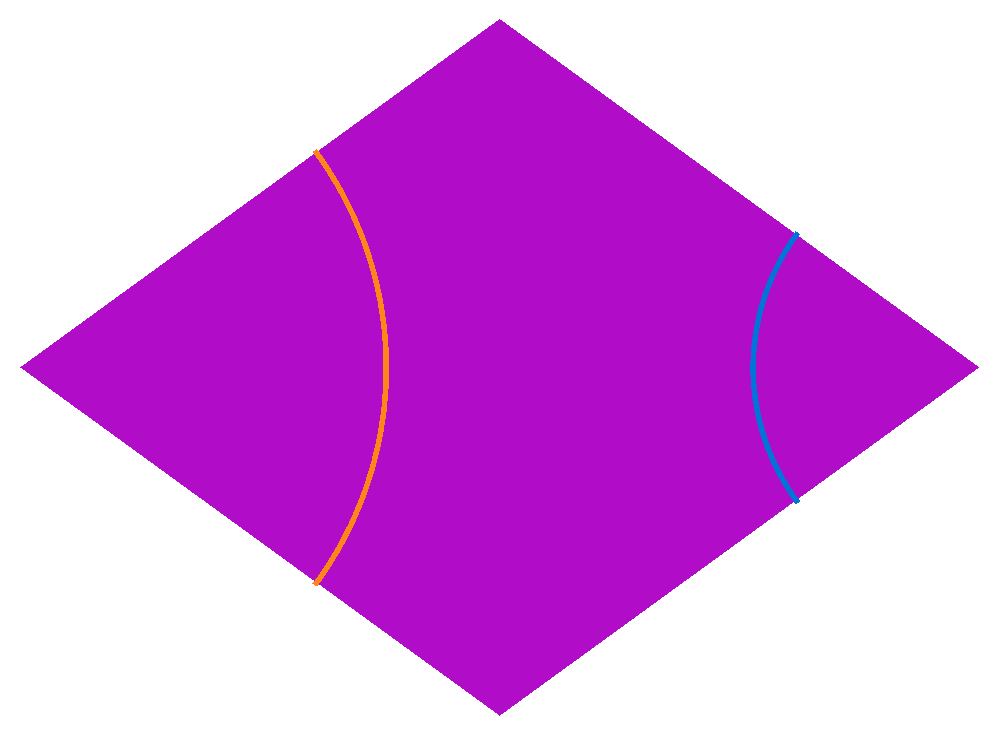
\includegraphics[scale=0.5]{RhombFat}}
                \caption{Thick Penrose Rhomb}
                \label{fig:ThickRhomb}
        \end{subfigure}\hfill
        \begin{subfigure}[b]{0.5\textwidth}
        \centering
                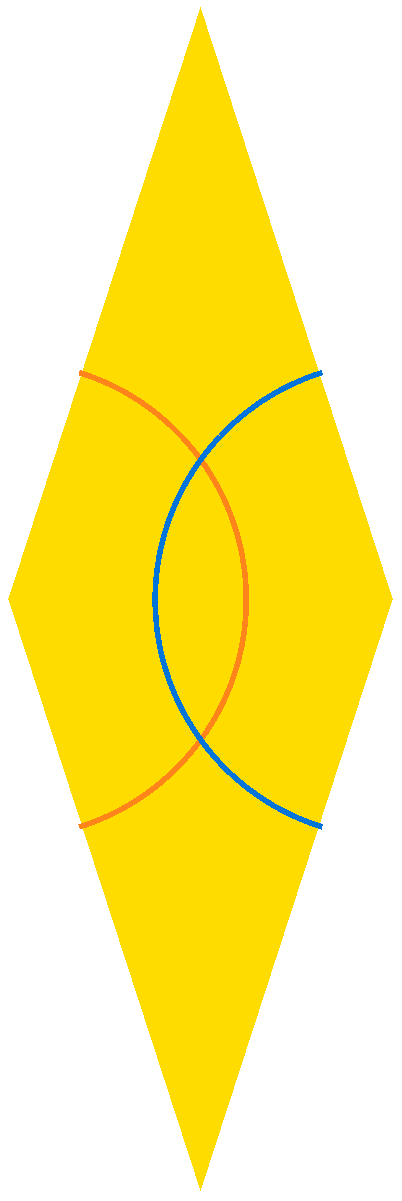
\includegraphics[scale=0.6]{RhombSkinny}
                \caption{Thin Penrose Rhomb}
                \label{fig:ThinRhomb}
        \end{subfigure}   
                \caption*{ \centering Penrose Rhombs from Robinson triangles. Blue and Orange curves illustrate matching rules.}
                \label{fig:JustRhombs}     
        \end{subfigure}
        \caption{Penrose Rhombs are generated by reflecting the Robinson triangles across their bases. The Rhombs with an edge-matching criterion, illustrated by the blue and orange curves, form an aperiodic protoset.}
        \label{fig:Rhombs}
\end{figure}

Now that we have seen the Penrose rhombs protoset, and the criteria which allow two tiles to meet, we can investigate how to construct valid tilings. Before continuing, however, it is important to note that the fact that a protoset admits a tiling does not guarantee that any valid arrangement of those prototiles can be continued to an infinite tiling. The Penrose tiling features a notable difficulty in procedurally constructing tilings one tile at a time due to the non-locality of tiling growth, this will be discussed shortly. Though, to motivate the consideration of Penrose tiling despite the frustration of non-locality, I will provide a theorem now which will be proven later.

\begin{mythm}
The Penrose Rhombs protoset, with matching rules, admits a tiling of the plane.
\end{mythm}

\subsection{Non-Local Growth}
\subsection{Constructing the Penrose Tiling}
\subsubsection{Substitution Construction}
Despite non-locality, Penrose and Conway showed that we can construct arbitrarily large tilings by repeated application of substitution rules.

To clearly understand the substitution rules on the rhombs, we will first demonstrate the substitution of the constituent Robinson triangles (Fig.\ref{fig:RobSubs})

\begin{figure}[H]
        \centering
        \begin{subfigure}[t]{\textwidth}
        \begin{subfigure}[t]{0.4\textwidth}
                \centering
               \raisebox{9px}{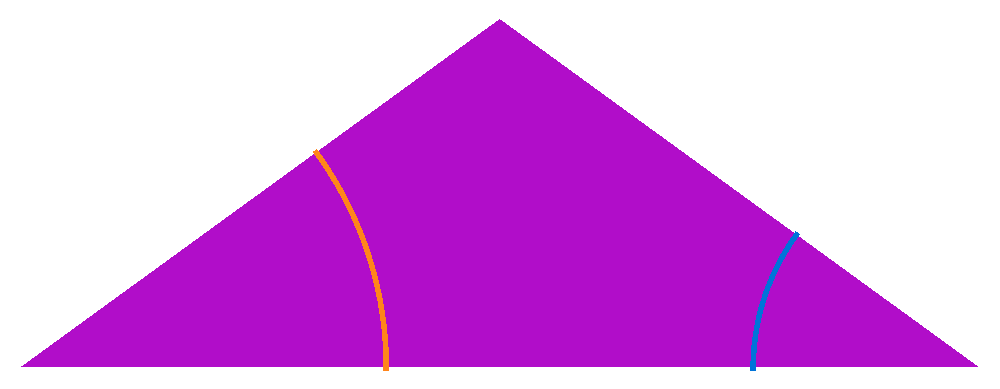
\includegraphics[scale=0.4]{RobinsonFat}}
        \end{subfigure}\hfill \raisebox{30px}{\huge$\rightarrow$} \hfill%
        ~ %add desired spacing between images, e. g. ~, \quad, \qquad, \hfill etc.
          %(or a blank line to force the subfigure onto a new line)
        \begin{subfigure}[t]{0.4\textwidth}
                \centering
                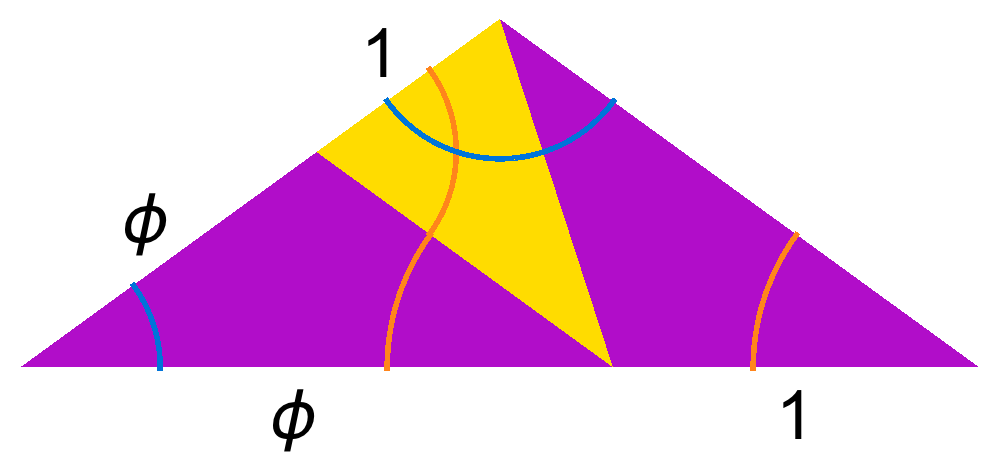
\includegraphics[scale=0.4]{RobFatSub}
        \end{subfigure}
        \caption{Substitution rule for Thick Robinson triangle}
        \label{fig:RobSubThick}
        \end{subfigure}
        ~ %add desired spacing between images, e. g. ~, \quad, \qquad, \hfill etc.
          %(or a blank line to force the subfigure onto a new line)
          
        \begin{subfigure}[b]{\textwidth}
        \begin{subfigure}[b]{0.4\textwidth}
        \centering
		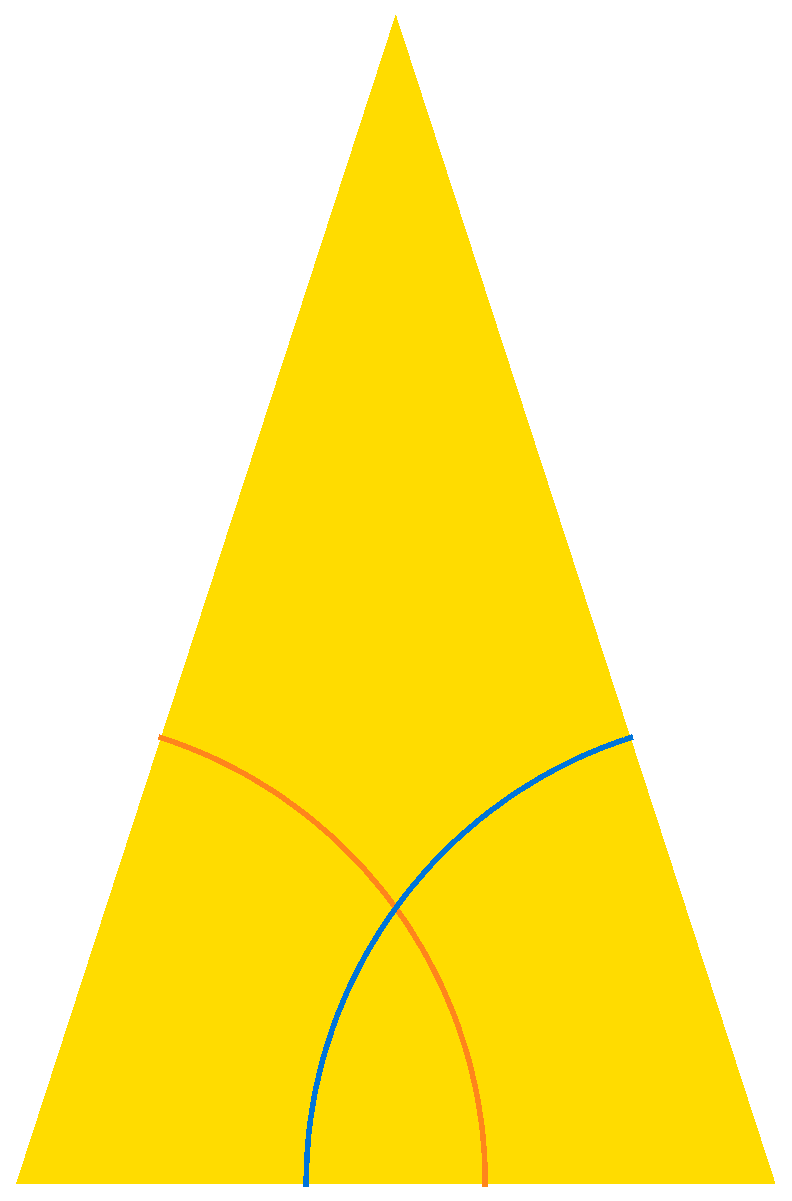
\includegraphics[scale=0.3]{RobinsonSkinny}
        \end{subfigure}\hfill \raisebox{30px}{\huge$\rightarrow$} \hfill
        \begin{subfigure}[b]{0.4\textwidth}
        \centering
                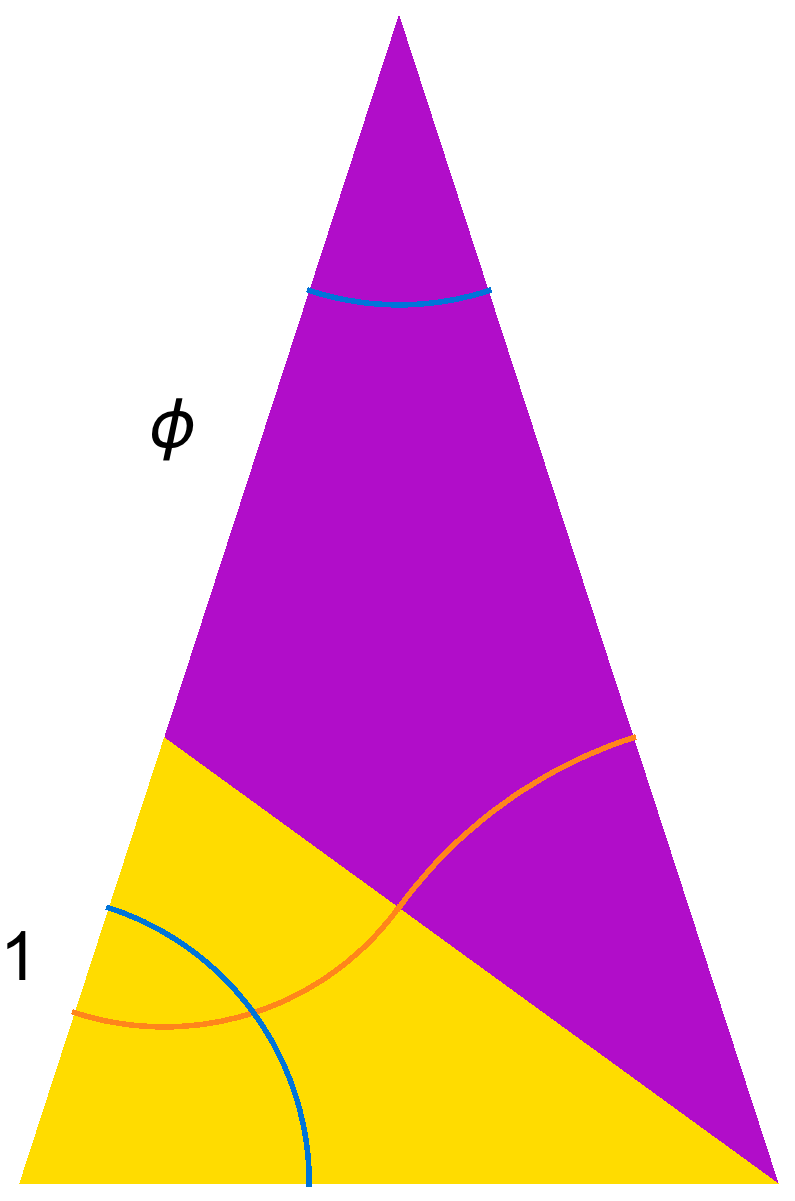
\includegraphics[scale=0.3]{RobSkinnySub}
        \end{subfigure}   
        \caption{Substitution rule for Thick Robinson triangle}
        \label{fig:RobSubThin}
        \end{subfigure}
        \caption{Substitution rules demonstrated on Robinson triangles. The substitution fragments each Robinson triangle into Robinson sub-triangles. The vertices of these sub-triangles are given such that the edges of the substituted triangle are divided according to the Golden ratio. The ratios of these divided edges are labeled accordingly. Note that these substitutions produce valid arrangements as per the edge-matching rules, illustrated by the orange and blue curves.}
        \label{fig:RobSubs}
\end{figure}

Recall that these Robinson triangles generate Penrose Rhombs by reflection across their bases (Fig.\ref{fig:Rhombs}). With that in mind, consider the above substitution applied to the Rhombs, such that each constituent Robinson triangle composing the Rhomb undergoes substitution as above. These substitution rules, applied to the Penrose Rhombs, is known as the process of \textbf{deflation}.

\begin{figure}[H]
        \centering
        \begin{subfigure}[t]{\textwidth}
        \begin{subfigure}[t]{0.4\textwidth}
                \centering
               \raisebox{30px}{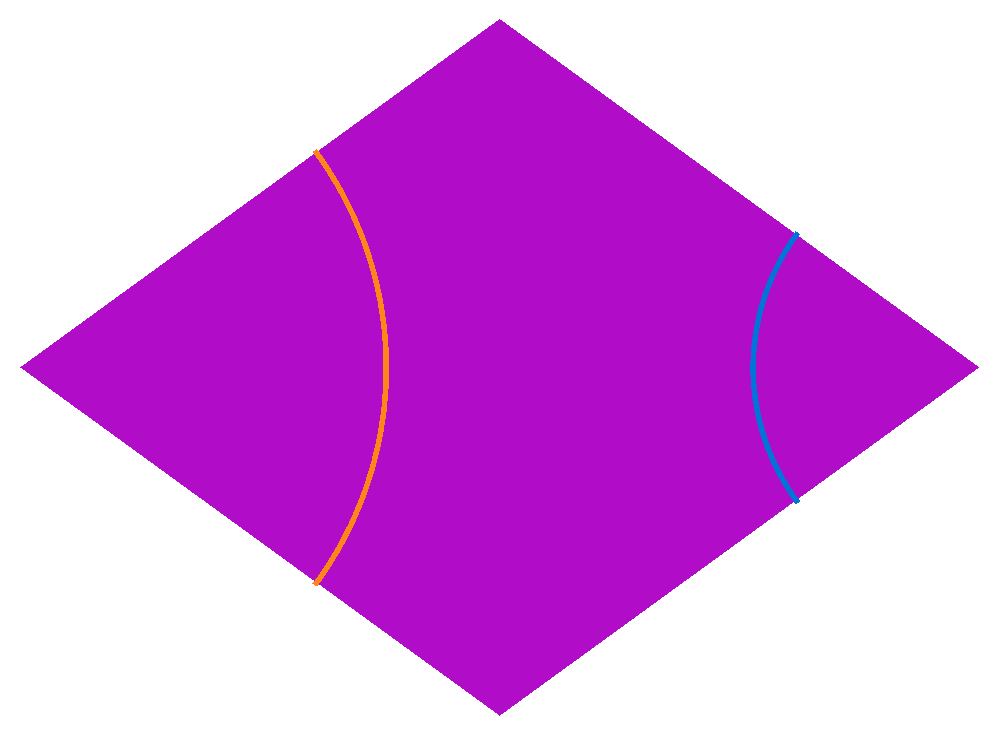
\includegraphics[scale=0.4]{RhombFat}}
        \end{subfigure}\hfill \raisebox{75px}{\huge$\rightarrow$} \hfill%
        ~ %add desired spacing between images, e. g. ~, \quad, \qquad, \hfill etc.
          %(or a blank line to force the subfigure onto a new line)
        \begin{subfigure}[t]{0.4\textwidth}
                \centering
                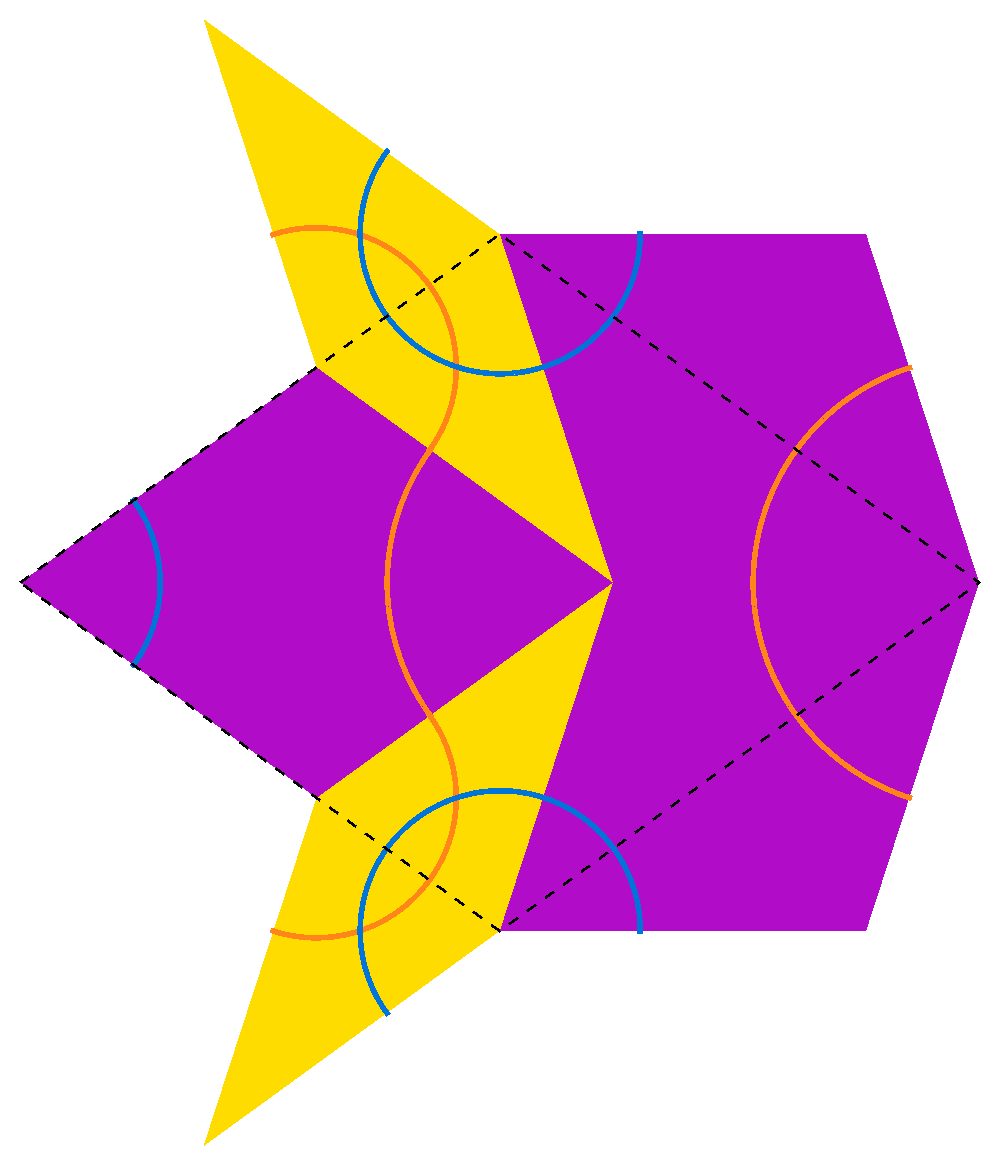
\includegraphics[scale=0.4]{RhombFatSub}
        \end{subfigure}
        \caption{Deflation rule for Thick Penrose Rhomb}
        \label{fig:RhombSubThick}
        \end{subfigure}
        ~ %add desired spacing between images, e. g. ~, \quad, \qquad, \hfill etc.
          %(or a blank line to force the subfigure onto a new line)
          
        \begin{subfigure}[b]{\textwidth}
        \begin{subfigure}[b]{0.4\textwidth}
        \centering
		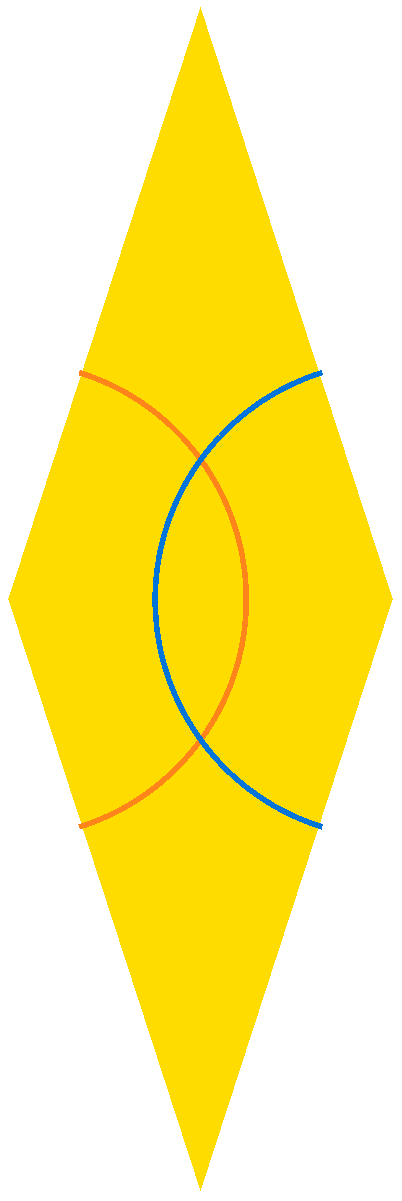
\includegraphics[scale=0.4]{RhombSkinny}
        \end{subfigure}\hfill \raisebox{75px}{\huge$\rightarrow$} \hfill
        \begin{subfigure}[b]{0.4\textwidth}
        \centering
                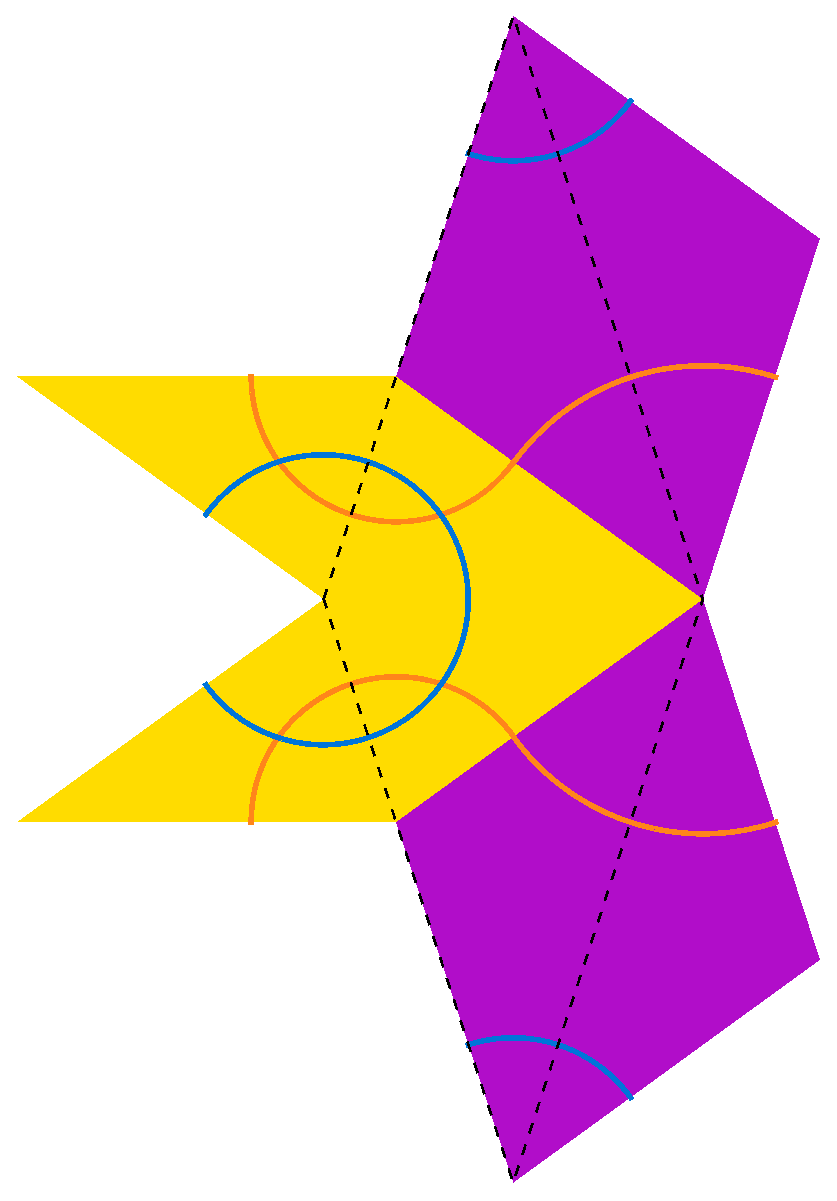
\includegraphics[scale=0.4]{RhombSkinnySub}
        \end{subfigure}   
        \caption{Deflation rule for Thin Penrose Rhomb}
        \label{fig:RobSubThin}
        \end{subfigure}
        \caption{Deflation rules of the Penrose Rhombs. Pre-substituted rhomb is illustrated with dashed black lines. Note that these substitutions produce valid arrangements as per the edge-matching rules, illustrated by the orange and blue curves.}
        \label{fig:RobSubs}
\end{figure}

This substitution process can be used to generate arbitrarily large Penrose tilings through a complementary process, called \textbf{inflation}. Following a series of deflation substitutions, the generated tiling is then `inflated' such that the deflated rhombuses are scaled to the same size as the original, pre-deflated rhombuses. Notice that a single application of the deflation rule scales the composite rhombi by a factor of $\frac{1}{\phi}$. This means that, after $n$ iterations of the deflation process, the resulting rhombs can be scaled, or inflated, by a factor of $\phi^n$ to return them to the original rhombus size. We can see in Figures \ref{fig:ThickDeflate} and \ref{fig:ThinDeflate} that iterations of the deflation process produce increasingly complex patterns. 

\begin{figure}[H]
\centering
\begin{tabular}{cc}
	        \begin{subfigure}[b]{0.4\textwidth}
	        \centering
	        \raisebox{30px}{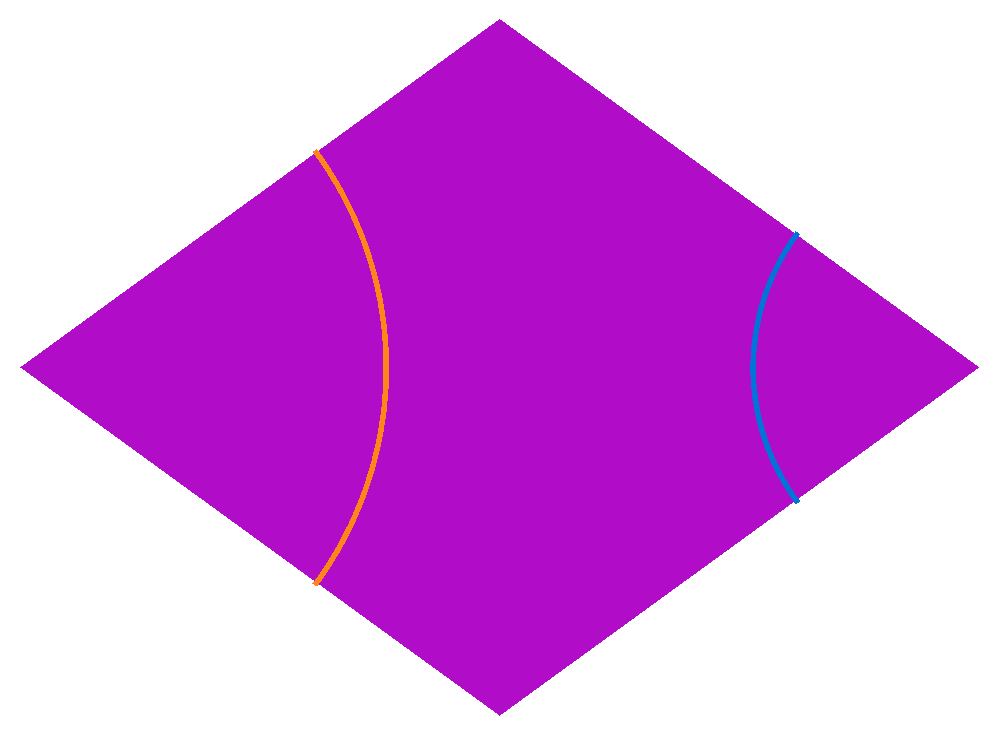
\includegraphics[scale=0.4]{FatInflation0}}
	        \end{subfigure}   &
            \begin{subfigure}[b]{0.4\textwidth}
             \centering
             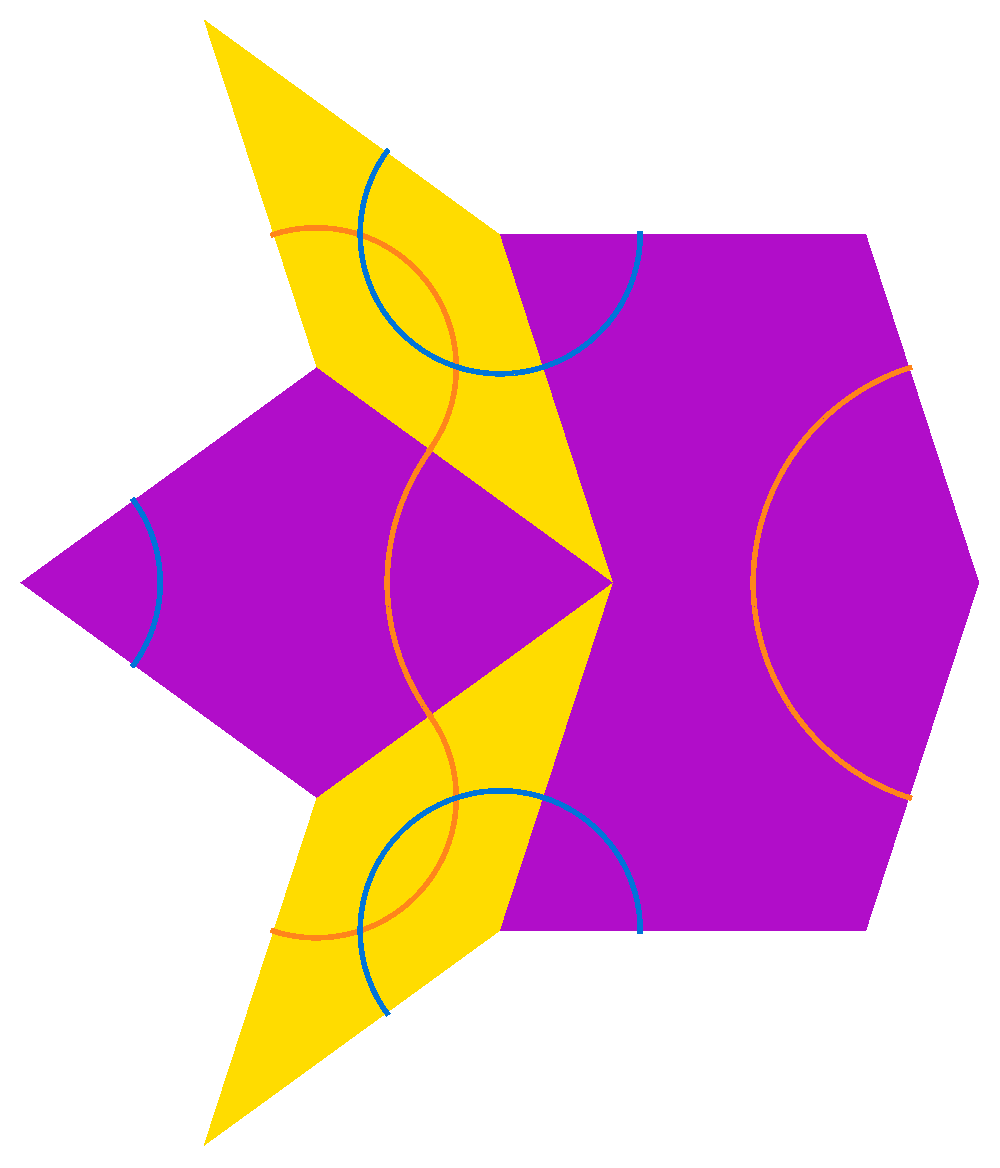
\includegraphics[scale=0.4]{FatInflation1}
             \end{subfigure}   \\
	       	 \begin{subfigure}[b]{0.4\textwidth}
             \centering
             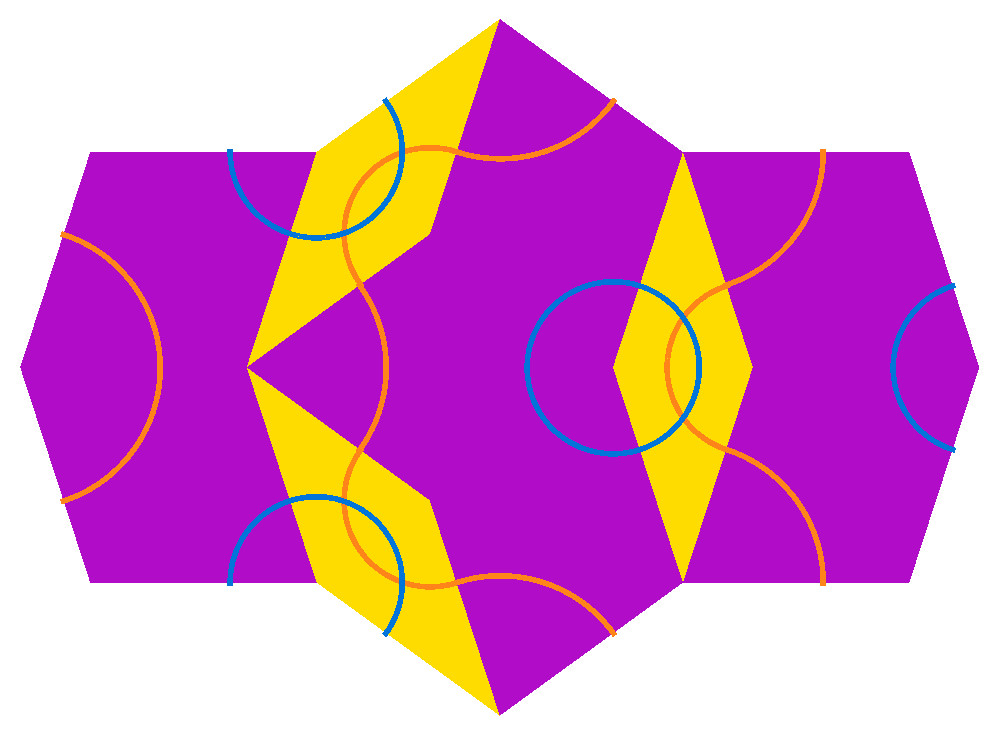
\includegraphics[scale=0.4]{FatInflation2}
             \end{subfigure}   &
             \begin{subfigure}[b]{0.4\textwidth}
             \centering
             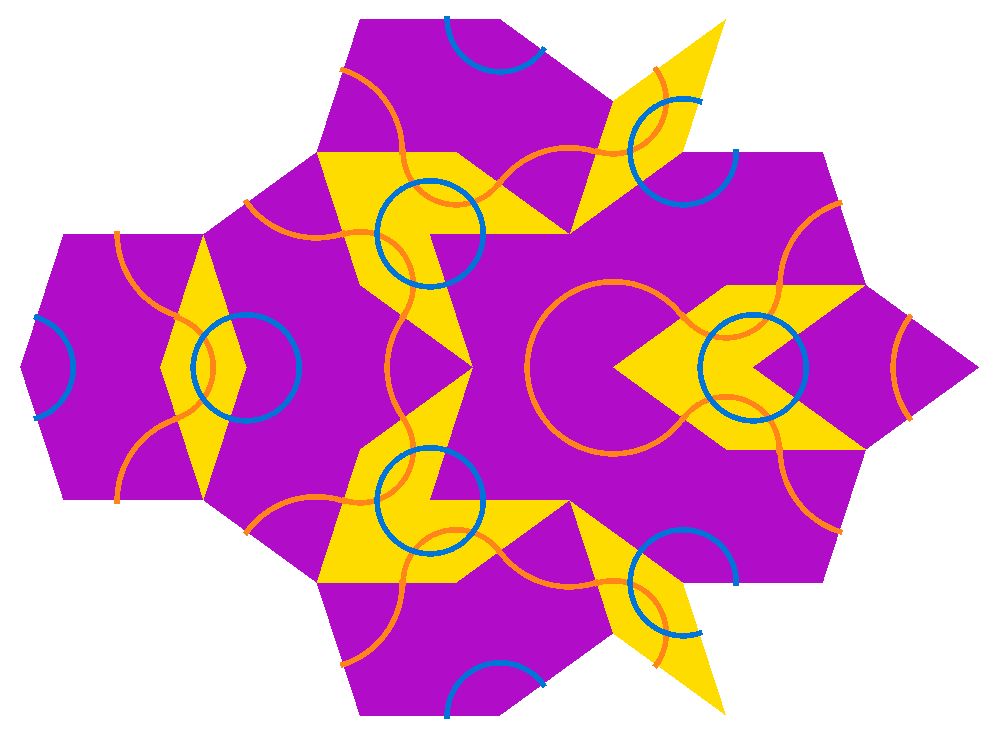
\includegraphics[scale=0.4]{FatInflation3}
             \end{subfigure}   \\
             \begin{subfigure}[b]{0.4\textwidth}
             \centering
             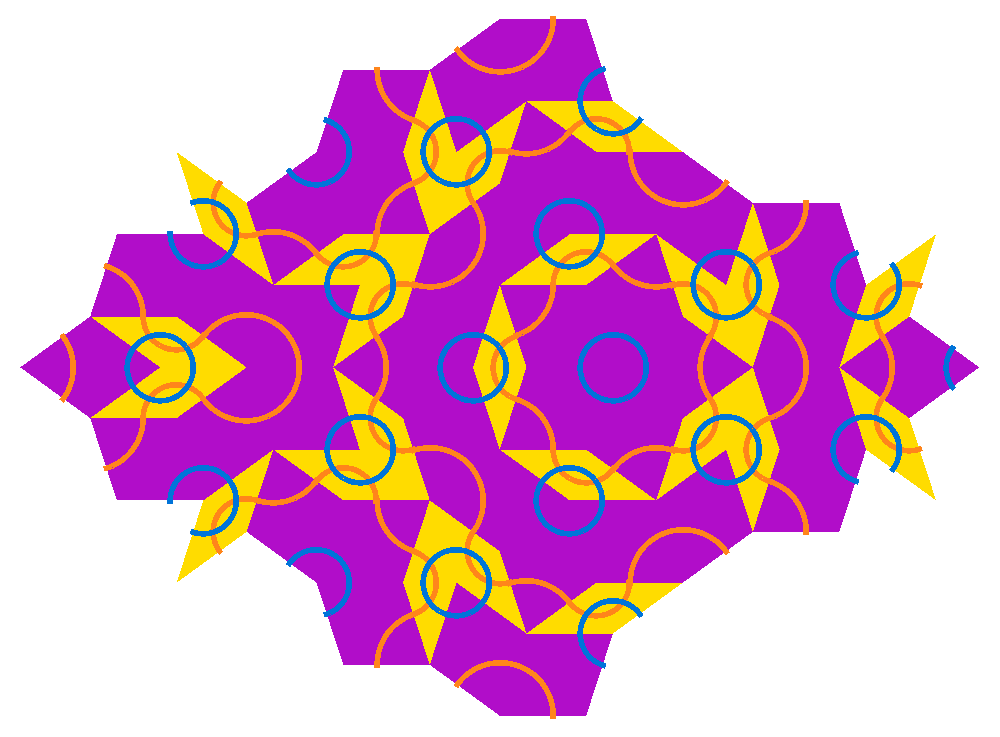
\includegraphics[scale=0.4]{FatInflation4}
             \end{subfigure}   &
             \begin{subfigure}[b]{0.4\textwidth}
             \centering
             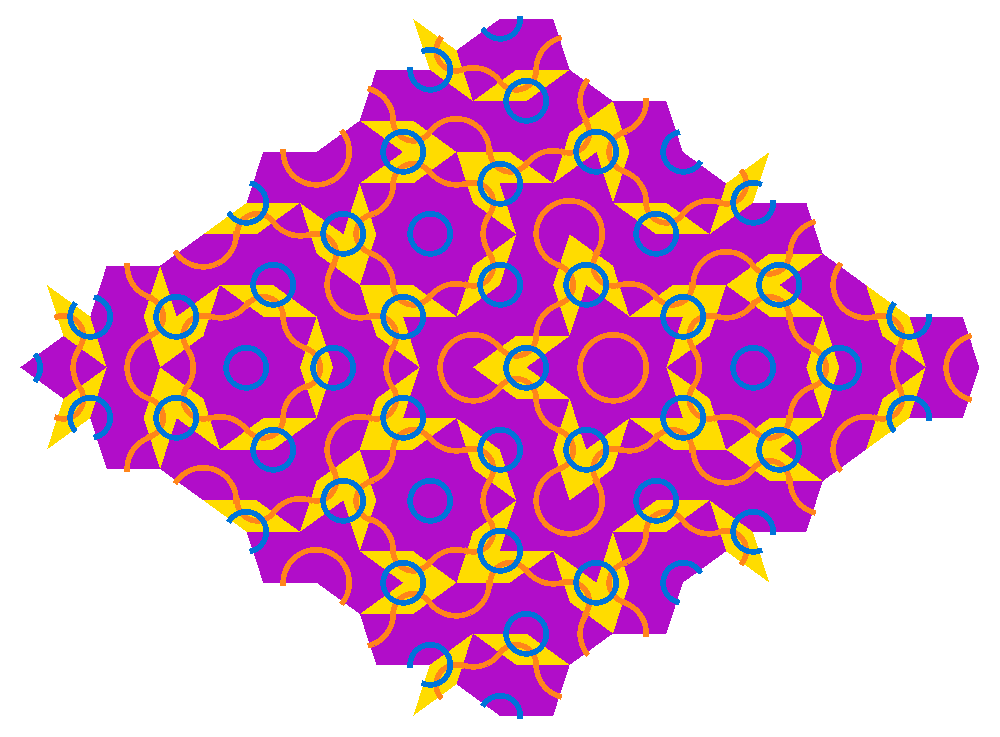
\includegraphics[scale=0.4]{FatInflation5}
             \end{subfigure}   \\
\end{tabular}
\caption{Five successive iterations of the deflation process applied to the Thick Rhombus.}
\label{fig:ThickDeflate}
	\end{figure}

\begin{figure}[H]
\centering
\begin{tabular}{cc}
	        \begin{subfigure}[b]{0.4\textwidth}
	        \centering
	        \raisebox{0px}{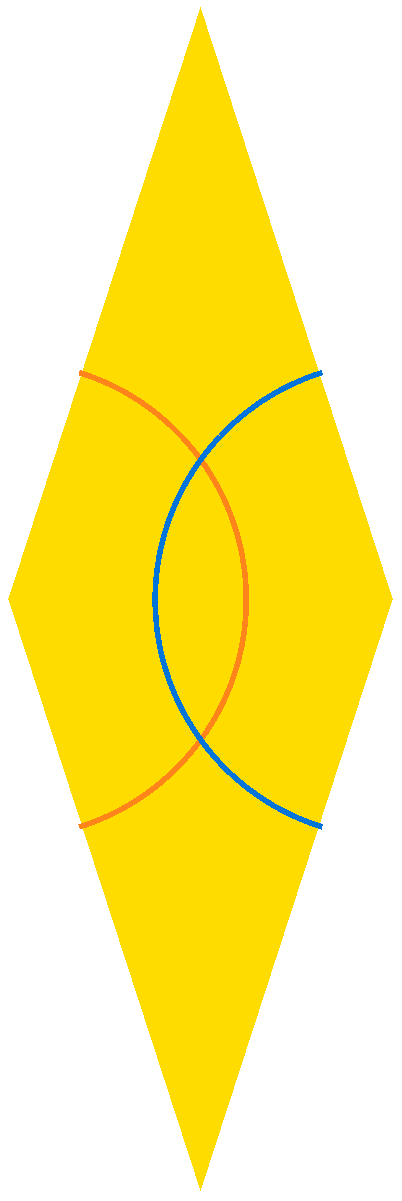
\includegraphics[scale=0.4]{SkinnyInflation0}}
	        \end{subfigure}   &
            \begin{subfigure}[b]{0.4\textwidth}
             \centering
             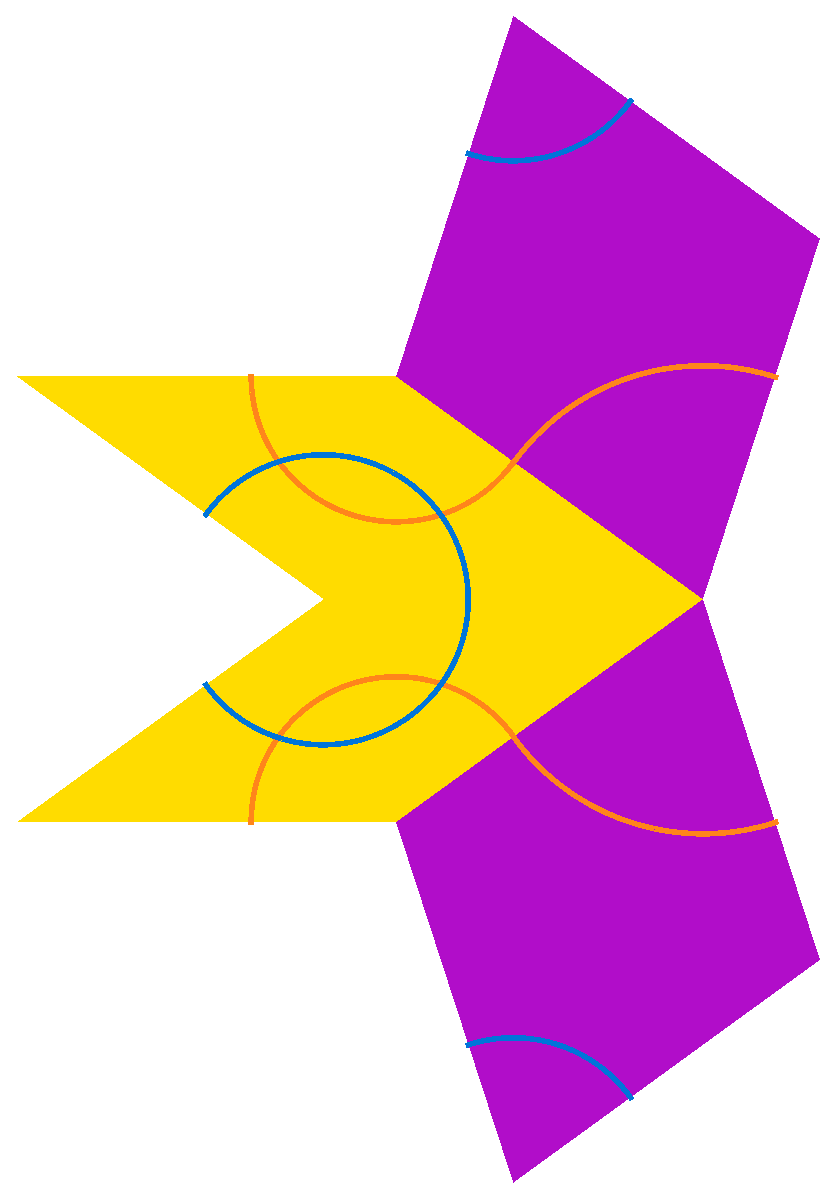
\includegraphics[scale=0.4]{SkinnyInflation1}
             \end{subfigure}   \\
	       	 \begin{subfigure}[b]{0.4\textwidth}
             \centering
             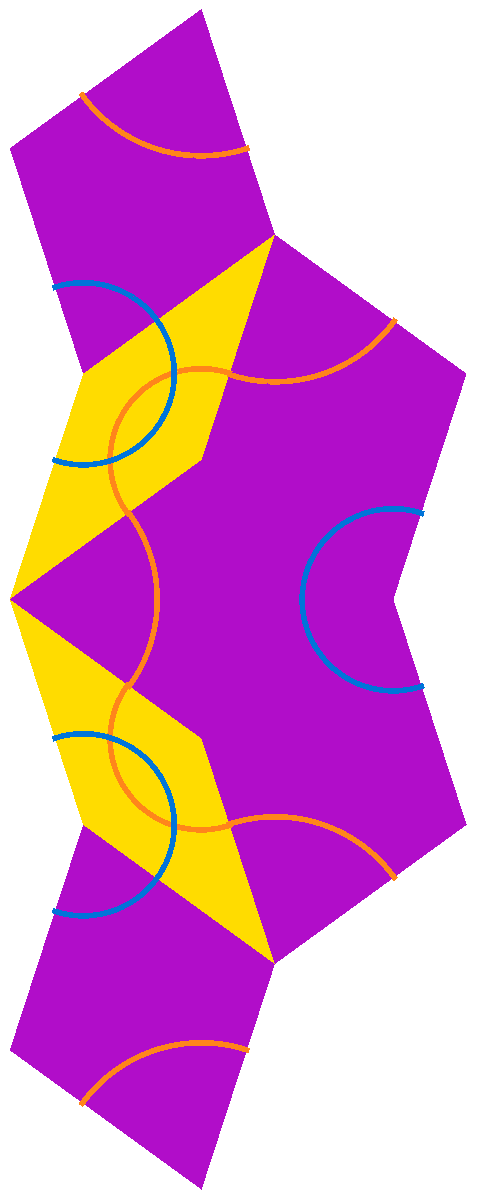
\includegraphics[scale=0.4]{SkinnyInflation2}
             \end{subfigure}   &
             \begin{subfigure}[b]{0.4\textwidth}
             \centering
             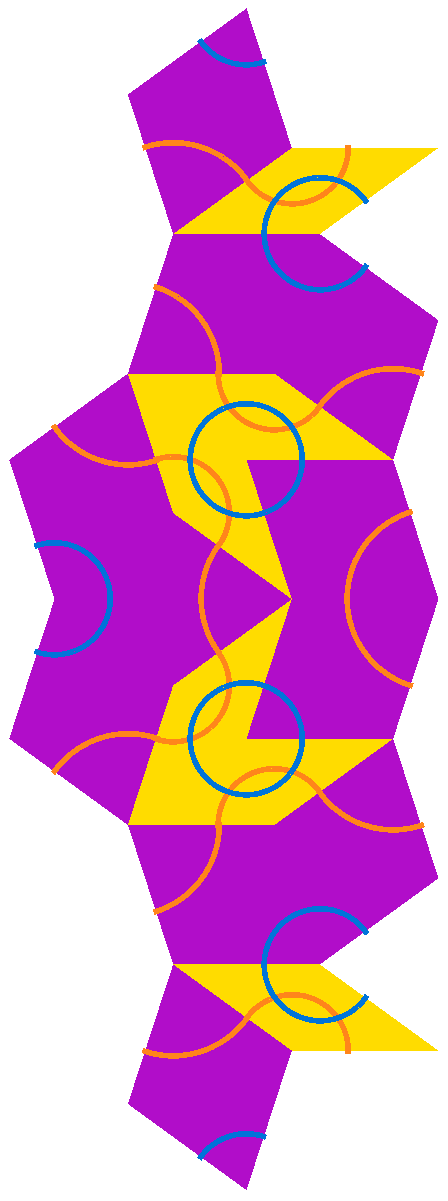
\includegraphics[scale=0.4]{SkinnyInflation3}
             \end{subfigure}   \\
             \begin{subfigure}[b]{0.4\textwidth}
             \centering
             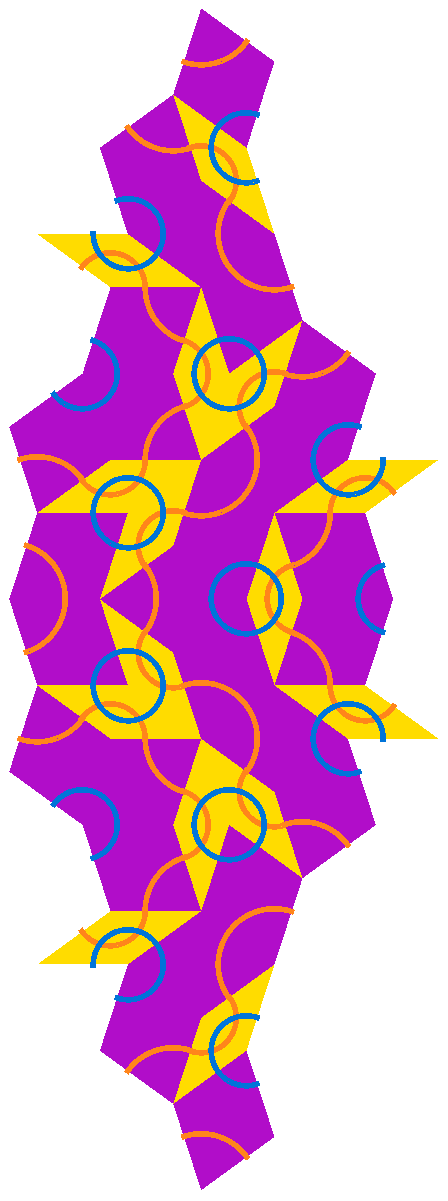
\includegraphics[scale=0.4]{SkinnyInflation4}
             \end{subfigure}   &
             \begin{subfigure}[b]{0.4\textwidth}
             \centering
             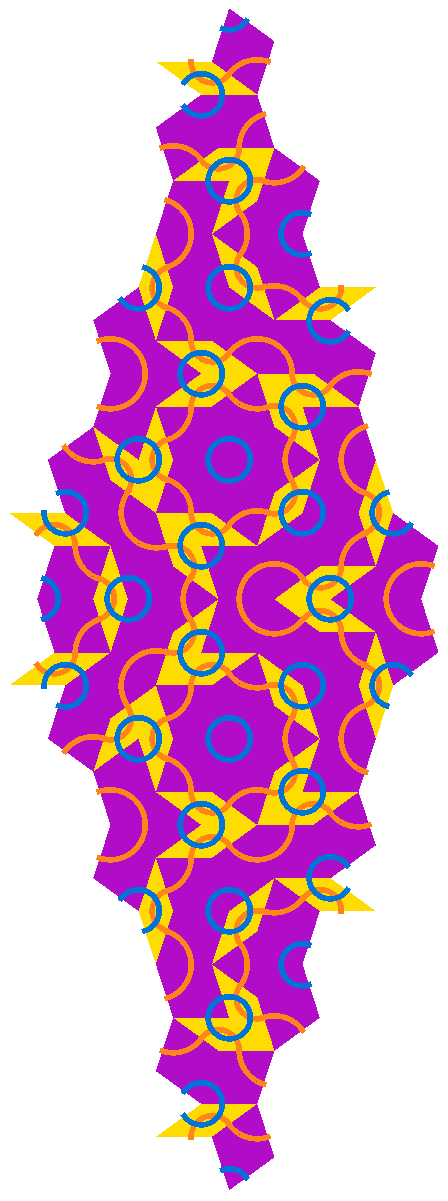
\includegraphics[scale=0.4]{SkinnyInflation5}
             \end{subfigure}   \\
\end{tabular}
\caption{Five successive iterations of the deflation process applied to the Thin Rhombus.}
\label{fig:ThinDeflate}
	\end{figure}
	
Consider again that under inflation each of the thick and thin rhombi in the deflated patterns will be scaled back to the original rhombi size. Further, consider that this substitution process can be iterated arbitrarily many times, generating a tiling that is arbitrarily large. 

Also, notice that even after successive applications of the deflation substitution, the resulting tiling is still valid under the initial matching rules. Again, in Figures \ref{fig:ThickDeflate} and \ref{fig:ThinDeflate} this is illustrated by the continuity of the orange and blue edge-matching curves.

\subsubsection{Up-Down Construction}
\subsubsection{Projective Construction}
\subsection{Extension Theorem}

\section{Features of Penrose Tiling}
\subsection{No Translational Symmetry}
\subsection{Five-fold Rotational Symmetry}
\begin{mythm}
No tiling can have more than one center of fivefold rotational symmetry.
\label{symthm}
\end{mythm}

\begin{figure}[H]
	\centering
	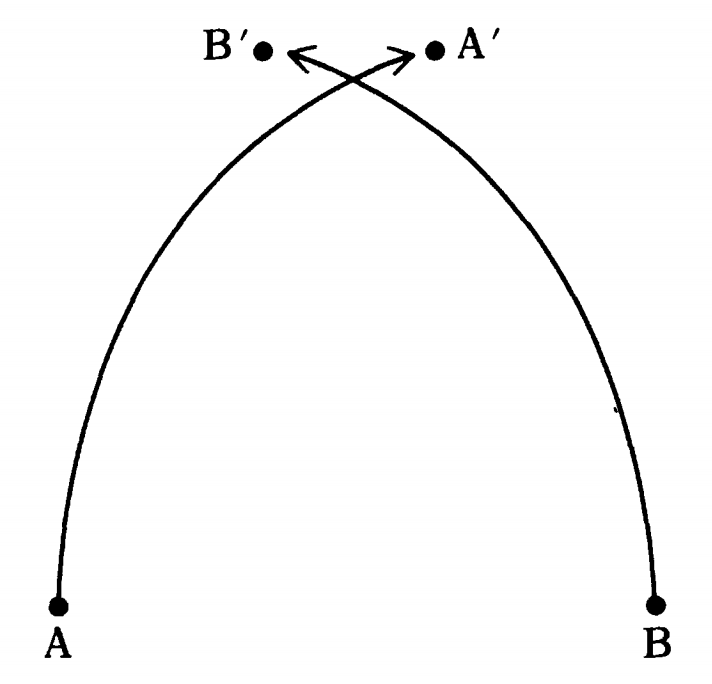
\includegraphics[width=0.4\textwidth]{proof}
    \caption{Barlow's Proof that no tiling can have more than one center of fivefold symmetry.}
    \label{fig:fivefoldproof}
\end{figure}

Conway provides a proof of this, attributed to Peter Barlow \cite{Gardner1997}.

\begin{proof}
Suppose in order to derive a contradiction that a tiling $\mathcal{T}$ has more than one center of fivefold symmetry.\\
Choose two centers, A and B, such that they are the nearest possible centers. \\
Rotate $\mathcal{T}$ counter-clockwise by $\frac{2\pi}{5}$ about $A$, bringing $B$ to $B'$, (see Fig.\ref{fig:fivefoldproof}).\\
Rotate $\mathcal{T}$ clockwise by $\frac{2\pi}{5}$ about $B$, bringing $A$ to $A'$.\\
A and B are centers of fivefold symmetry, so the tiling will overlap identically.\\
$\implies$ $A'$ and $B'$ are centers of fivefold symmetry.\\
But $A'$ and $B'$ are closer than $A$ and $B$.\\
This contradicts hypothesis that $A$ and $B$ are nearest centers of fivefold symmetry.\\
$\therefore$ By contradiction, $\mathcal{T}$ can only have one center of fivefold symmetry.
\end{proof}

We've shown that no tiling can have more than one center of fivefold symmetry. Using this theorem we can show, further, that even one center of fivefold symmetry is impossible if the tiling is periodic. First, consider these properties of periodic tilings:

\begin{myprop}
A periodic tiling can be subdivided into countably infinitely many regions, $\mathcal{R}$, which are congruent by translation such that
\begin{enumerate}
\item Two regions have no common interior points: $\mathring{\mathcal{R}_i} \cap  \mathring{\mathcal{R}_j}=\emptyset$ if $i\neq j$
\item The union of regions is exactly the tiling: $\bigcup_{i=1}^\infty \mathcal{R}_i = \mathcal{T}=\mathbb{E}^n$
\item For any two regions, $\mathcal{R}_i$ and $\mathcal{R}_j$, there is a translation that takes  $\mathcal{R}_i$ to $\mathcal{R}_j$. This translation also admits symmetry, carrying the entire tiling onto itself. \label{periodprop3}
\end{enumerate}
\label{periodprop}
\end{myprop}

\begin{mylem}
If tiling $\mathcal{T}$ is periodic, then it cannot have any centers of fivefold symmetry.
\end{mylem}
The proof of this is identical to the proof of Theorem \ref{symthm}.
\begin{proof}
Suppose in order to derive a contradiction that A is a center of fivefold rotational symmetry.\\
Since $\mathcal{T}$ is periodic, by condition \ref{periodprop3} of Property \ref{periodprop}, we see that there must be countably infinitely many centers of fivefold symmetry.\\
By Theorem \ref{symthm}, this is impossible.\\
$\therefore$ By contradiction, periodic tilings have no centers of fivefold symmetry.
\end{proof}

We have shown that fivefold symmetry is incompatible with periodic tilings. For this reason, the admittance of a single center fivefold symmetry is related to the aperiodicity of a tiling. As we will see, centers of fivefold symmetry are possible in Penrose tilings. 

\subsection{Local Isomorphism}
\subsection{Ratio of Prototiles}


\section{Collin's Paths on Penrose Tiles}
\subsection{Path Generation Rules}
\subsection{Types of Paths}






\nocite{Penrose1979,Ogawa1999,Kepler1997,DeBruijn1990,DeBruijn1989,DeBruijn1981,Conway1986}
\bibliographystyle{plain}
\bibliography{bibliography}



\end{document}


\section{Introduction}
\subsection{Theory of Periodic Tiling}

In 1619, Kepler discovered the third law of planetary motion which he described in his book \textit{Harmonices Mundi} (The Harmonies of the World). In this work, Kepler also provides the first mathematical treatment of plane tiling by regular polygons. Primarily, he shows that only 3 regular polygons; triangles, squares, and hexagons; are able to completely tile the plane, that is, without overlap or gaps (Fig. \ref{fig:regular}). Further, Kepler experimented with tilings produced by combinations of polygon tiles (Fig. \ref{fig:combo}). While patterns of this kind have been known to the ancients, featured widely in art and architecture, it was Kepler who first provided a mathematical framework with which to discuss these tiling patterns. One aspect of this treatment is the symmetry of the tiling. 

We can describe the tiling patterns generally by the symmetries which they admit. In planar tilings there are four fundamental types of symmetry: 
\begin{enumerate}
\item A tiling has \textbf{rotational} symmetry if it can be rotated a non-trivial angle about a point and overlap itself identically.
\item A tiling has \textbf{reflection} symmetry if it can be mirrored across a line and overlap itself identically. 
\item A tiling has \textbf{translational} symmetry if it can be shifted by some non-trivial distance in a direction and overlap itself identically.
\item A tiling has \textbf{glide} symmetry if it can be translated some distance, then reflected about a line, and overlap itself identically.
\end{enumerate}

Using the notion of translational symmetry, we can introduce a new property of plane tiling, periodicity. A tiling is said to be \textbf{periodic} if it admits translational symmetry. The tilings in Fig. \ref{fig:regular} and Fig. \ref{fig:combo} are all periodic, but is it possible to make a tiling pattern which is not periodic? Well, actually it's quite easy. Consider the square tiling in Fig. \ref{fig:square} but with each column shifted up and down by some random decimal amount. This tiling of jostled squares would completely tile the plane, but since the squares are all randomly shifted there's no way we could translate the entire plane so that it overlaps itself. This is an example of a tiling pattern which does not have the periodic property, we call these patterns aperiodic. 




\begin{figure}
        \centering
        \begin{subfigure}[hb]{0.3\textwidth}
                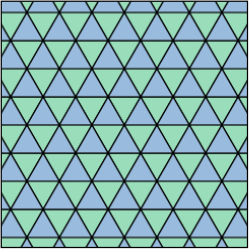
\includegraphics[width=\textwidth]{triangle}
                \caption{Tiling by triangles}
                \label{fig:triangle}
        \end{subfigure}%
        ~ %add desired spacing between images, e. g. ~, \quad, \qquad, \hfill etc.
          %(or a blank line to force the subfigure onto a new line)
        \begin{subfigure}[hb]{0.3\textwidth}
                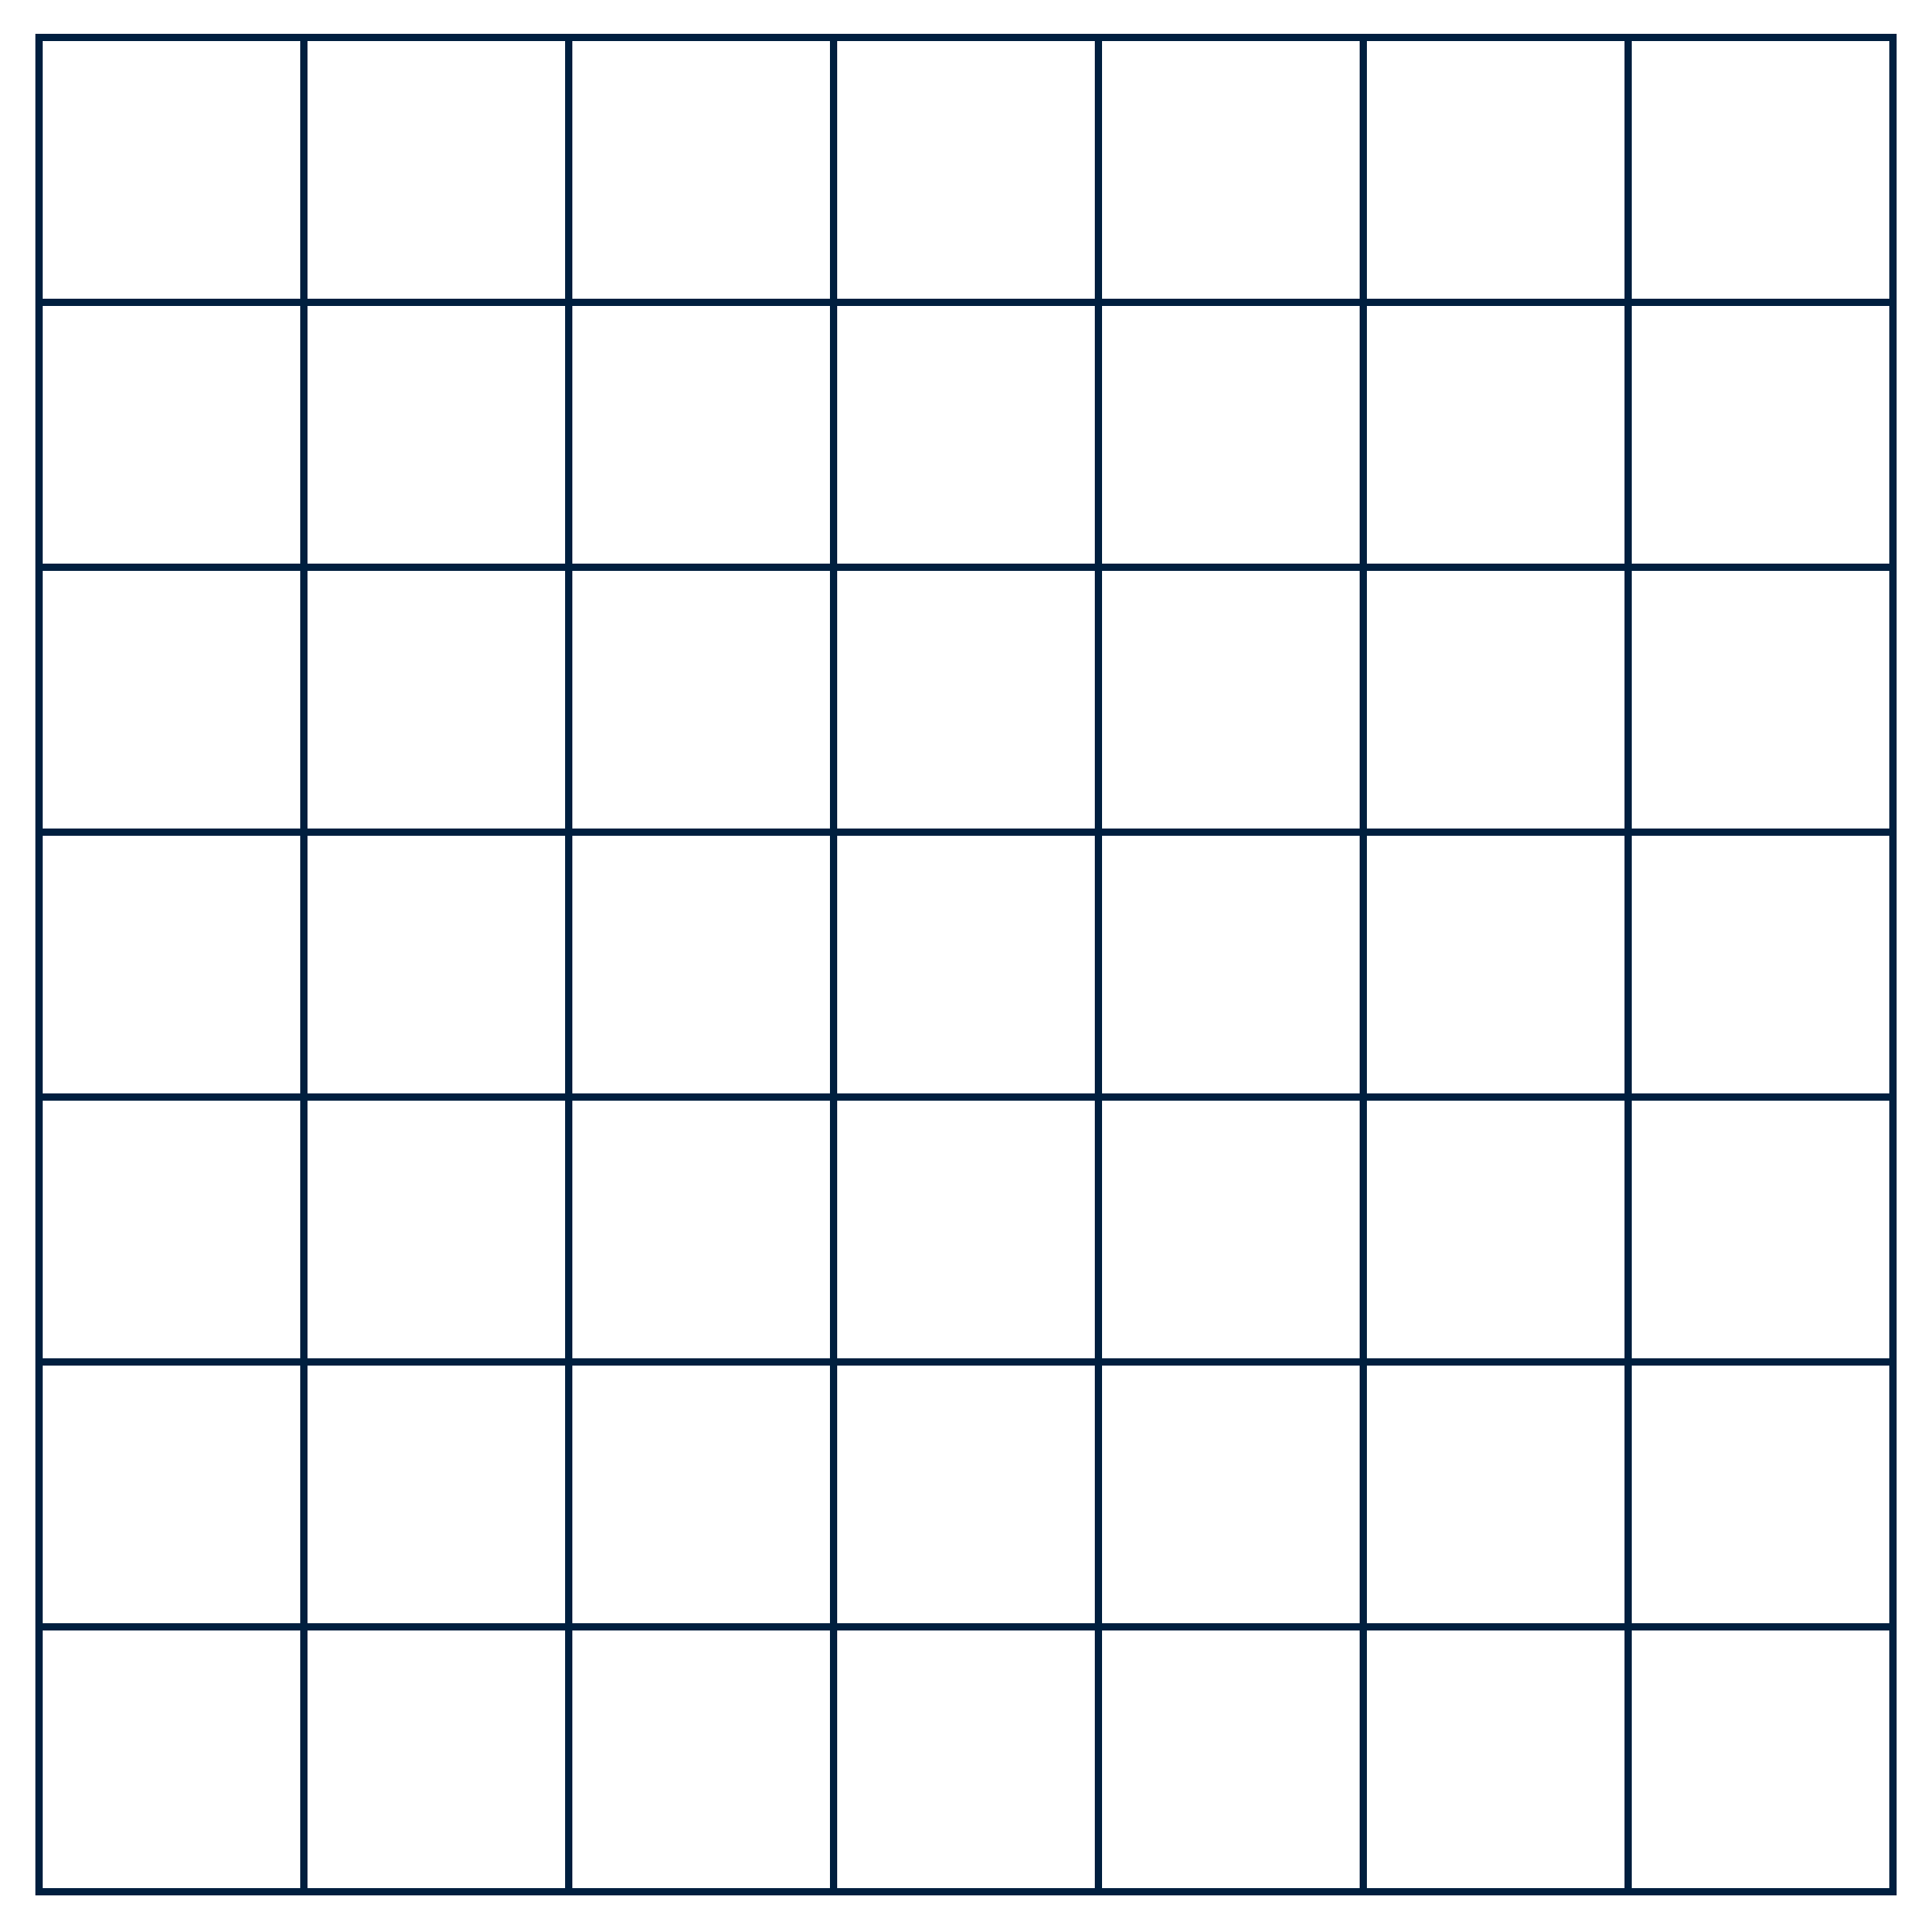
\includegraphics[width=\textwidth]{square}
                \caption{Tiling by squares}
                \label{fig:square}
        \end{subfigure}
        ~ %add desired spacing between images, e. g. ~, \quad, \qquad, \hfill etc.
          %(or a blank line to force the subfigure onto a new line)
        \begin{subfigure}[hb]{0.3\textwidth}
                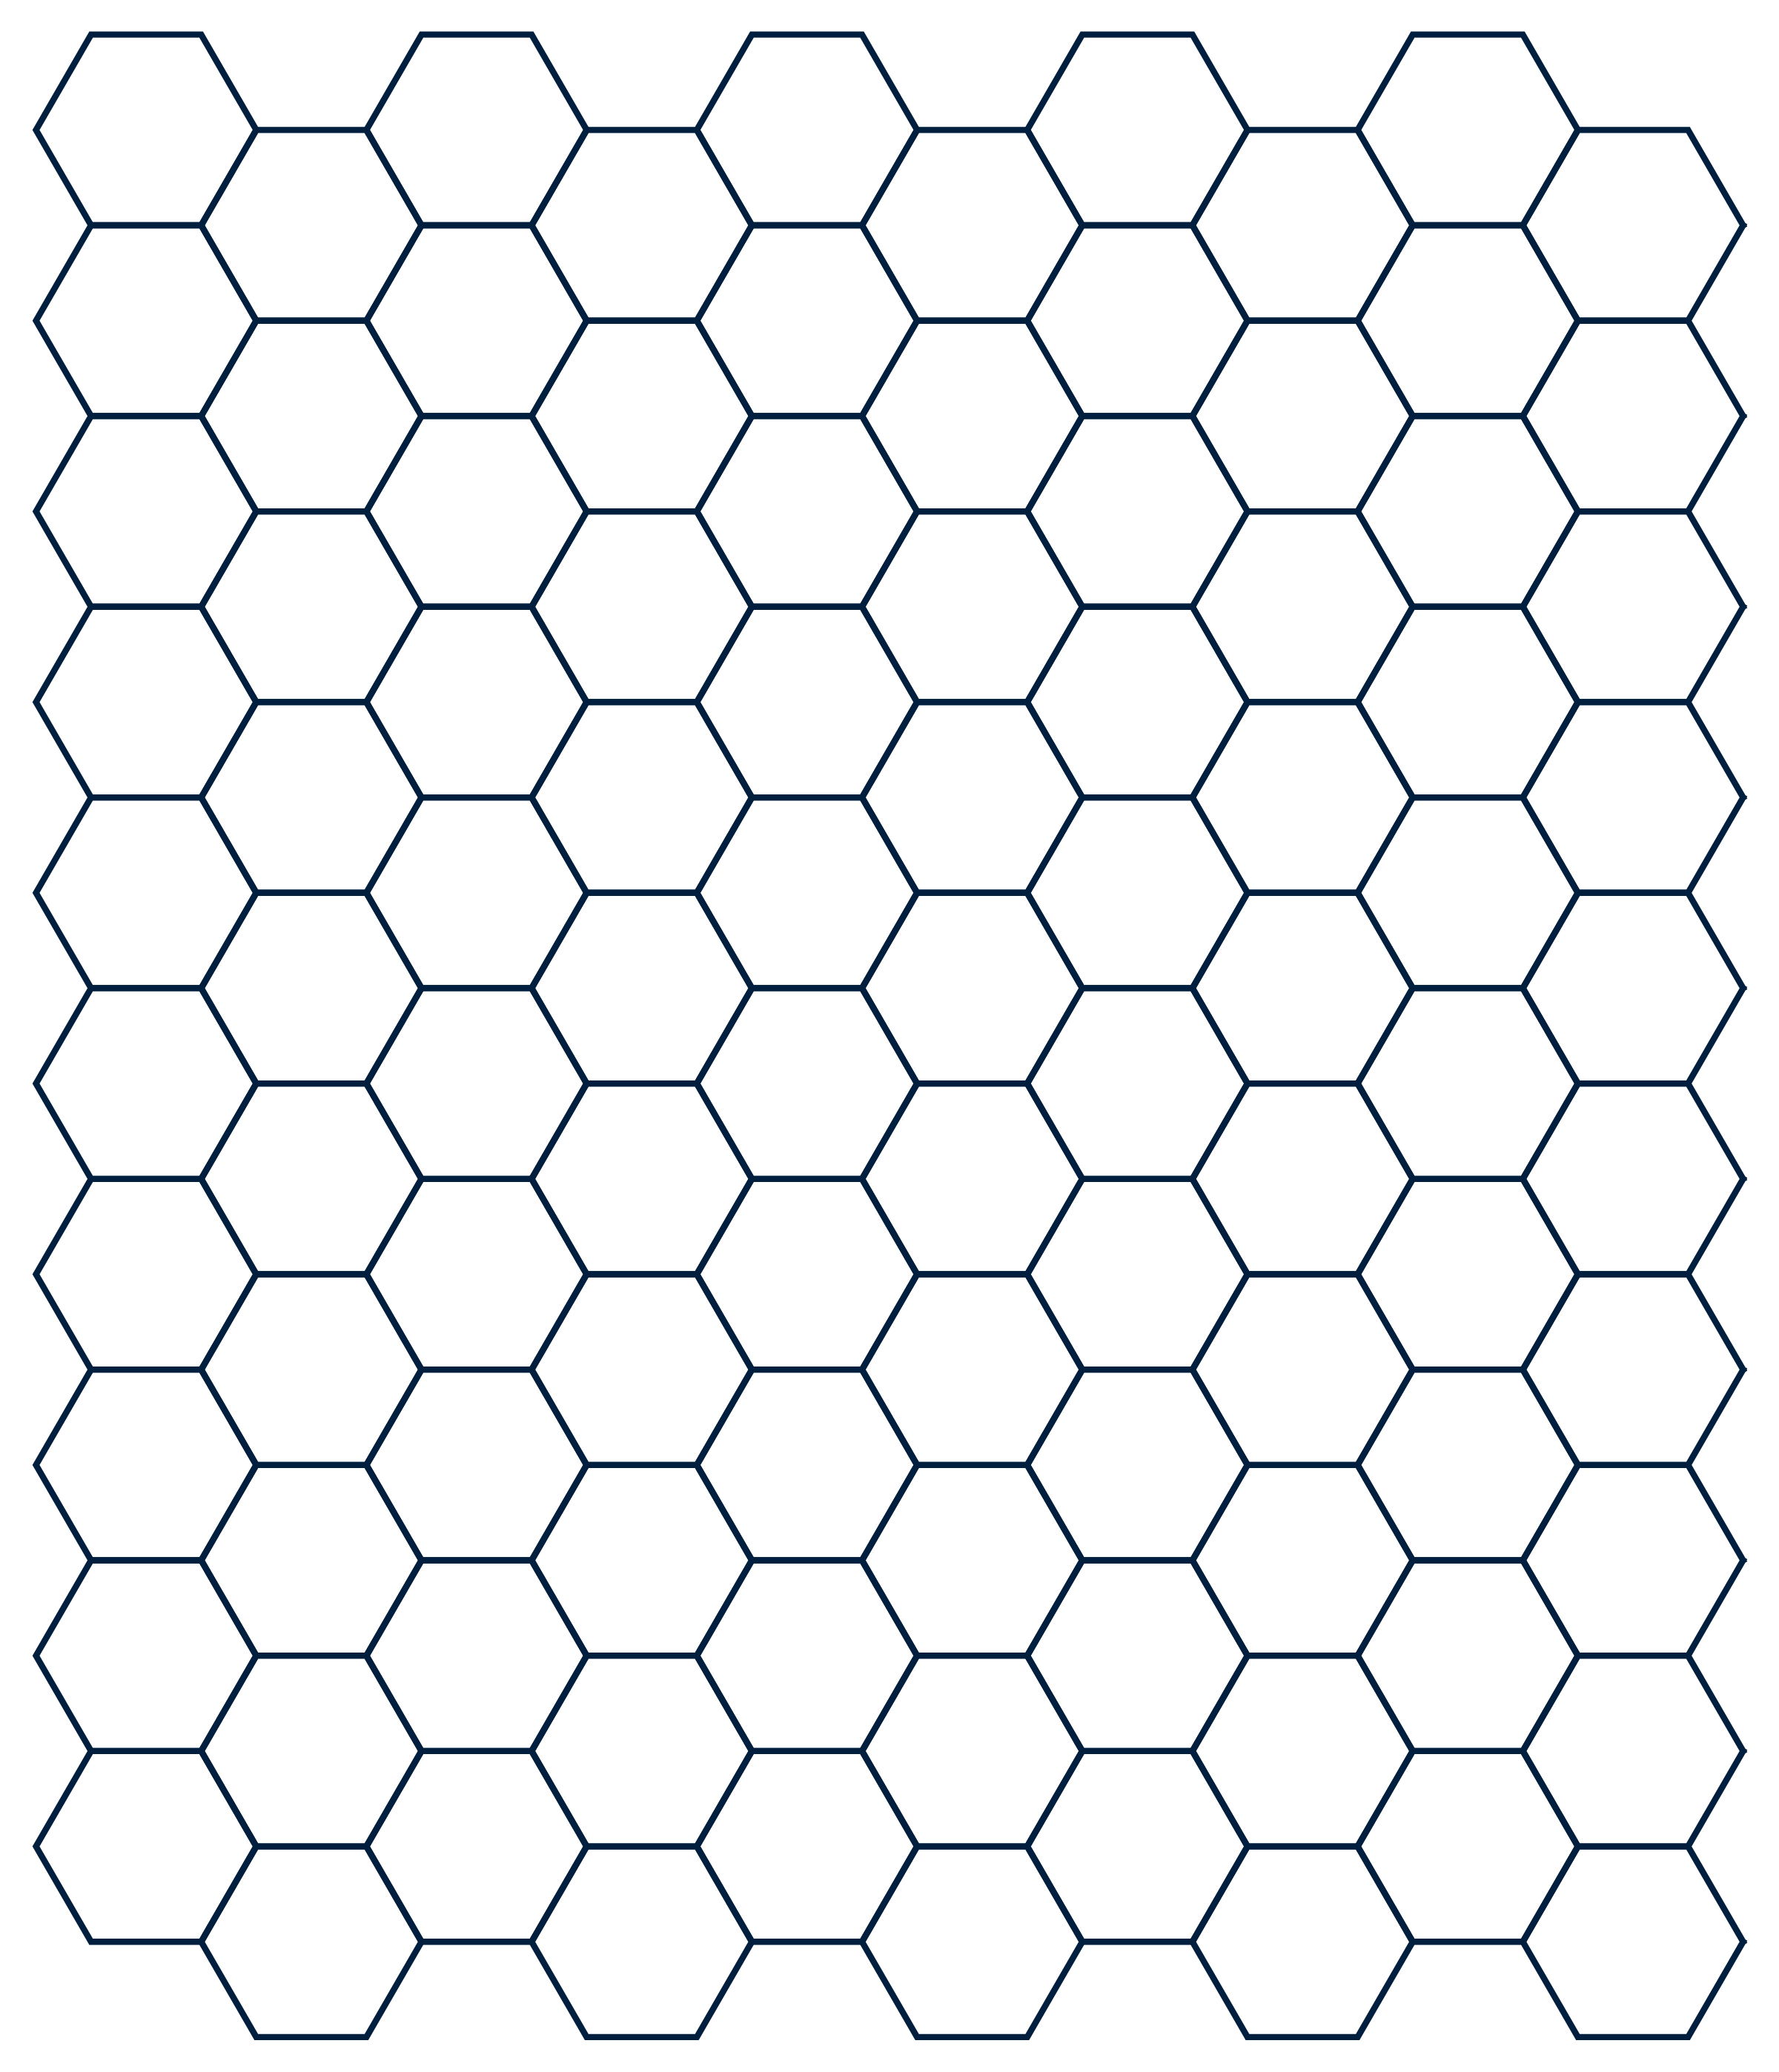
\includegraphics[width=\textwidth]{hexagon}
                \caption{Tiling by hexagons}
                \label{fig:hexagon}
        \end{subfigure}
        \caption{Regular tiling of the plane using single polygons}\label{fig:regular}
\end{figure}

\begin{figure}
        \centering
        \begin{subfigure}[hb]{0.3\textwidth}
                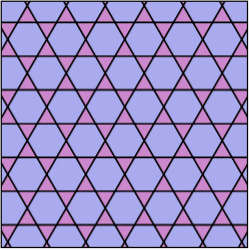
\includegraphics[width=\textwidth]{trihexagon}
                \caption{Trihexagonal }
                \label{fig:trihex}
        \end{subfigure}%
        ~ %add desired spacing between images, e. g. ~, \quad, \qquad, \hfill etc.
          %(or a blank line to force the subfigure onto a new line)
        \begin{subfigure}[hb]{0.3\textwidth}
                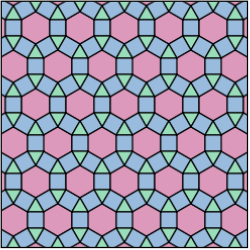
\includegraphics[width=\textwidth]{rhombitrihexagon}
                \caption{Rhombitrihexagonal}
                \label{fig:rhombitri}
        \end{subfigure}
        ~ %add desired spacing between images, e. g. ~, \quad, \qquad, \hfill etc.
          %(or a blank line to force the subfigure onto a new line)
        \begin{subfigure}[hb]{0.3\textwidth}
                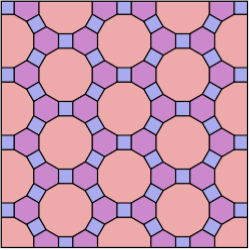
\includegraphics[width=\textwidth]{truncatedtrihexagon}
                \caption{Truncated trihexagon \textbf{}}
                \label{fig:trunctrihexagon}
        \end{subfigure}
        \caption{Periodic tiling of the plane using combination of polygons}\label{fig:combo}
\end{figure}

\subsection{History of Aperiodic Tiling}



\subsection{Definitions}



\subsection{The Forbidden Symmetry}
